\documentclass{cslthse-msc}
\usepackage[utf8]{inputenc}
\usepackage[english]{babel}
\usepackage{amsmath}
\usepackage{amsfonts}
\usepackage{amssymb}
\usepackage{amsthm}
%\usepackage{makeidx}
\usepackage{graphicx}
\usepackage[titletoc, header, page]{appendix}
\usepackage{hyperref}

\usepackage{float}
\usepackage{listings}

\lstset{ %
%  backgroundcolor=\color{white},   % choose the background color; you must add \usepackage{color} or \usepackage{xcolor}
  basicstyle=\footnotesize,        % the size of the fonts that are used for the code
  breakatwhitespace=false,         % sets if automatic breaks should only happen at whitespace
  breaklines=true,                 % sets automatic line breaking
  captionpos=b,                    % sets the caption-position to bottom
%  commentstyle=\color{mygreen},    % comment style
%  deletekeywords={...},            % if you want to delete keywords from the given language
  escapeinside={\%*}{*)},          % if you want to add LaTeX within your code
  extendedchars=true,              % lets you use non-ASCII characters; for 8-bits encodings only, does not work with UTF-8
  frame=single,                    % adds a frame around the code
  keepspaces=true,                 % keeps spaces in text, useful for keeping indentation of code (possibly needs columns=flexible)
%  keywordstyle=\color{blue},       % keyword style
%  language=Octave,                 % the language of the code
%  morekeywords={*,...},            % if you want to add more keywords to the set
  numbers=left,                    % where to put the line-numbers; possible values are (none, left, right)
  numbersep=10pt,                   % how far the line-numbers are from the code
  numberstyle=\tiny\color{mygray}, % the style that is used for the line-numbers
  rulecolor=\color{black},         % if not set, the frame-color may be changed on line-breaks within not-black text (e.g. comments (green here))
  showspaces=false,                % show spaces everywhere adding particular underscores; it overrides 'showstringspaces'
  showstringspaces=false,          % underline spaces within strings only
  showtabs=false,                  % show tabs within strings adding particular underscores
  stepnumber=2,                    % the step between two line-numbers. If it's 1, each line will be numbered
%  stringstyle=\color{mymauve},     % string literal style
  tabsize=2,                       % sets default tabsize to 2 spaces
  title=\lstname                   % show the filename of files included with \lstinputlisting; also try caption instead of title
}

%\geometry{showframe}

\author{
	Anton Fagerberg \\
	{\normalsize \href{mailto:ada10afa@student.lu.se}{\texttt{ada10afa@student.lu.se}}}
}

\title{Work in progress title}
\subtitle{A {\LaTeX} class}
\company{Jayway}
\supervisor{Roger Henriksson, \href{mailto:Roger.Henriksson@cs.lth.se}{\texttt{Roger.Henriksson@cs.lth.se}}}
\examiner{Görel Hedin, \href{mailto:Gorel.Hedin@cs.lth.se}{\texttt{Gorel.Hedin@cs.lth.se}}}

\date{\today}
%\date{February 18, 2014}

\acknowledgements{
If you want to thank people, do it here, on a separate right-hand page. Both the U.S. \textit{acknowledgments} and the British \textit{acknowledgements} spellings are acceptable.

We would like to thank Lennart Andersson for his feedback on this template.
}

\theabstract{
This document describes the Master's Thesis format for the theses carried out at 
the Department of Computer Science, Lund University. 

Your abstract should capture, in English, the whole thesis with focus on the problem and solution in 150 words. It should be placed on a separate right-hand page, with an additional \textit{1cm} margin on both left and right. Avoid acronyms, footnotes, and references in the abstract if possible.

Leave a \textit{2cm} vertical space after the abstract and provide a few keywords relevant for your report. Use five to six words, of which at most two should be from the title.
}

\keywords{MSc, template, report, style, structure}

%% Only used to display font sizes
\makeatletter
\newcommand\thefontsize[1]{{#1 \f@size pt\par}}
\makeatother
%%%%%%%%%%


\begin{document}
\makefrontmatter

\chapter{Performance issues with HTTP 1.1}
Hypertext Transfer Protocol (HTTP) is an application protocol for distributed, collaborative, hypermedia information systems\cite{http-info}. The first standard version of HTTP/1.1 was released in January 1997\cite{rfc2068}. The next version, HTTP/2 (originally named HTTP/2.0), is expected to be finalised in 2015 (ändra här om det publiceras innan ex-jobbet är klart). Although HTTP/2 addresses several of the HTTP/1.1 performance issues, it is reasonable to assume that it will take many years before HTTP/2 fully replaces HTTP/1.1 as the protocol used on all web servers and middle-boxes such as proxies and firewalls --- and even longer for many legacy systems and clients used in the enterprise environments. It is therefore relevant to  acknowledge and mitigate the performance issues related to HTTP 1.1, even many years after the release of HTTP/2.

\section{Headers}
\label{headers}

It is common in modern web applications to send a lot of HTTP requests toward one or many back-end APIs. These requests can be very small, such as a PUT request to update a single field, but the actual payload of a HTTP requests can also be considered small in many cases when it is compared to the total amount of data being transfered. There are typically plenty of headers along with every HTTP request and these headers can be a substantial amount of every request and may therefore end up being the performance bottle neck --- especially if a lot of small requests has to be transmitted often.

As an example, consider the Instagram API\cite{instagram_api} which has an end-point where you can get information about a certain user account. The response is serialised in JSON format. 

Suppose client was built which is supposed to show details about, for example, your 10 most followed friends. We can benchmark how making 10 separate API requests would differ, in transmitted HTTP data size, from how it would behave if we could fetch all 10 users with one request.

\begin{figure}[H]
  \centering
    \begin{lstlisting}
{
    "data": {
        "id": "1574083",
        "username": "snoopdogg",
        "full_name": "Snoop Dogg",
        "profile_picture": "http://distillery[...]",
        "bio": "This is my bio",
        "website": "http://snoopdogg.com",
        "counts": {
            "media": 1320,
            "follows": 420,
            "followed_by": 3410
        }
    }
}
    \end{lstlisting}
  \caption{User data response from the Instagram API encoded in JSON format.}
\end{figure}

HTTP requests can be benchmarked using cURL\cite{curl}. To make the requests authentic and look like they were made from an actual browser, we tell cURL to use the default headers provided by the browser Firefox. These headers includes among other things the browsers User-Agent, media types which are acceptable responses and so on. A local server running on port 9000 is used to simulate the the Instagram API in this particular example.

\begin{figure}[H]
  \centering
\begin{lstlisting}[breaklines=true]
curl --trace-ascii - 'http://localhost:9000/user/snoopdogg' -H 'Host: localhost:9000' -H 'User-Agent: Mozilla/5.0 (Macintosh; Intel Mac OS X 10.10; rv:36.0) Gecko/20100101 Firefox/36.0' -H 'Accept: text/html,application/xhtml+xml,application/xml;q=0.9,*/*;q=0.8' -H 'Accept-Language: en-US,en;q=0.5' --compressed -H 'Connection: keep-alive' -H 'Pragma: no-cache' -H 'Cache-Control: no-cache'
\end{lstlisting}
  \caption{The cURL command used in the benchmarks.}
\end{figure}

Performing this request will give us the following results:

\begin{figure}[H]
  \centering
\begin{lstlisting}[breaklines=true]
=> Send header, 355 bytes (0x163)
0000: GET /user/snoopdogg HTTP/1.1
001e: Accept-Encoding: deflate, gzip
003e: Host: localhost:9000
0054: User-Agent: Mozilla/5.0 (Macintosh; Intel Mac OS X 10.10; rv:36.
0094: 0) Gecko/20100101 Firefox/36.0
00b4: Accept: text/html,application/xhtml+xml,application/xml;q=0.9,*/
00f4: *;q=0.8
00fd: Accept-Language: en-US,en;q=0.5
011e: Connection: keep-alive
0136: Pragma: no-cache
0148: Cache-Control: no-cache
0161:
<= Recv header, 17 bytes (0x11)
0000: HTTP/1.1 200 OK
<= Recv header, 47 bytes (0x2f)
0000: Content-Type: application/json; charset=utf-8
<= Recv header, 21 bytes (0x15)
0000: Content-Length: 286
<= Recv header, 2 bytes (0x2)
0000:
<= Recv data, 286 bytes (0x11e)
\end{lstlisting}
  \caption{Results from cURL when sending an HTTP request to fetch one user. The actual response payload has been omitted.}
  \label{fig:headers_overhead}
\end{figure}

We can from the output in Figure~\ref{fig:headers_overhead} that 355 bytes are sent as request header data, 87 bytes are received as response header data (17 + 47 + 21 + 2) and the actual response payload is 286 bytes. This means 61\% of every request to this API end-point are nothing but header data.

Some of the header data is often required and it does contain useful information so we can't just discard it. But if we instead would expose one end-point where all ten users could be requested simultaneously with one HTTP request, and that end-point could return an array of JSON objects instead, then we would get away with only transmitting the header data once and not ten times.

\begin{figure}[H]
  \centering
\begin{lstlisting}[breaklines=true]
=> Send header, 446 bytes (0x1be)
0000: GET /users/snoopdog1,snoopdog2,snoopdog3,snoopdog4,snoopdog5,sno
0040: opdog6,snoopdog7,snoopdog8,snoopdog9,snoopdo10 HTTP/1.1
0079: Accept-Encoding: deflate, gzip
0099: Host: localhost:9000
00af: User-Agent: Mozilla/5.0 (Macintosh; Intel Mac OS X 10.10; rv:36.
00ef: 0) Gecko/20100101 Firefox/36.0
010f: Accept: text/html,application/xhtml+xml,application/xml;q=0.9,*/
014f: *;q=0.8
0158: Accept-Language: en-US,en;q=0.5
0179: Connection: keep-alive
0191: Pragma: no-cache
01a3: Cache-Control: no-cache
01bc:
<= Recv header, 17 bytes (0x11)
0000: HTTP/1.1 200 OK
<= Recv header, 47 bytes (0x2f)
0000: Content-Type: application/json; charset=utf-8
<= Recv header, 22 bytes (0x16)
0000: Content-Length: 2871
<= Recv header, 2 bytes (0x2)
0000:
<= Recv data, 2871 bytes (0xb37)
\end{lstlisting}
  \caption{Results from cURL when performing one HTTP request to fetch 10 users. The actual response payload has been omitted.}
  \label{fig:headers_overhead2}
\end{figure}

From the results in Figure~\ref{fig:headers_overhead2}, we can see that the size of the request headers has been increased from 355 to 446 bytes because of the longer URL which specifies all users to fetch. The response headers are increased with just one byte from 87 to 88 because of the increased \emph{Content-Length} field. This results in a total header size of 534 bytes. The response payload has increased from 286 bytes to 2871 bytes - about ten-fold which is expected since we request 10 users at once instead of one per request. A very small increase in data is added because of the array syntax in the JSON format. 

By not doing ten separate requests, and instead do one concatenated request, the overhead added as a result of all the headers have now been reduced from 61\% to 16\%. This number will scale accordingly to the number of requests concatenated --- the more requests concatenated, the lesser amount of overhead from HTTP headers.

\begin{figure}[H]
  \centering
    \begin{center}
      \begin{tabular}{ r | c | c }
        \textbf{\#} & \textbf{10 users, 10 request} & \textbf{10 users, 1 request} \\ \hline
        Total headers & 4,420 B & 534 B \\ \hline
        Total payload & 2,860 B & 2,871 B \\ \hline
        \% headers of total data & 61\% & 16\% \\ \hline
      \end{tabular}
    \end{center}
  \caption{Header and payload ratio when doing ten separate requests, compared to one concatenated request, to fetch all users.}
\end{figure}

The header data displayed in this example should be viewed as a lower bound. In practise, HTTP cookies, which are used for personalisation, analytics and session management, are also sent with every HTTP request as part of the headers and can add up to multiple kilobytes of protocol overhead for every single HTTP request\cite[page 200]{HPBN}.

This is one of the issues that may (ändra "may" om det stämmer när http2 släpps - kolla även HTTP compressions och säkerhetsproblem) be mitigated by using HTTP/2 which remembers which headers that has already been sent and therefore doesn't need to retransmit them on subsequent requests\cite[page 222]{HPBN}.

\section{Maximum TCP connections}
\label{max_tcp}
The HTTP/1.X protocol does not allow data to be multiplexed over the same connection\cite[p.194]{HPBN}. For this reason, most browser vendors has introduced a connection pool of six TCP connections per host (the HTTP/1.1 specification limits the pool to two connections\cite{rfc2616} per host, but modern browsers have refused to conform to this standard in order to decrease the load times).

A common way to deal with the connection limit is to use domain sharding. Since the limit of six TCP connections are on a host name basis, it is possible to create multiple subdomains to get around this limit. If the subdomains \{shard1, shard2, \ldots\}.example.com were created and they all pointed to the same server, then more than six TCP connections can be used in parallel at the same time to the same server from a browser. 

This approach is not without downsides as every new hostname requires a new DNS lookup, a TCP three-Way handshake and a TCP slow start which can have a negative impact on the load times\cite[page 199]{HPBN} --- just the DNS lookup typically takes 20-120 ms\cite[page 63]{HPWS}. Another problem with domain sharding is the fact that the browser always opens six connections per shard even if not all, or none of them are used. In addition, domain sharding can be a complicated manual process to set-up and it is hard to determine how many shards to use for optimal performance. When Yahoo investigated this problem they concluded that you should, as a rule of thumb, use at least two, but no more than four domain shards\cite{yahoo-performance-4}.

As an example, we can benchmark the impact of the connection pool limit when downloading thumbnails for an image gallery. Suppose we want to download 60 thumbnails, each encoded in base-64 format. The connection we are using in this example has a lot of bandwidth but suffers from high latency.

If all images were retrieved using one HTTP request per thumbnail, we can see in Figure~\ref{fig:tcp_bottleneck} that the six TCP connection limit will become a bottleneck.

\begin{figure}[H]
  \centering
    \begin{center}
      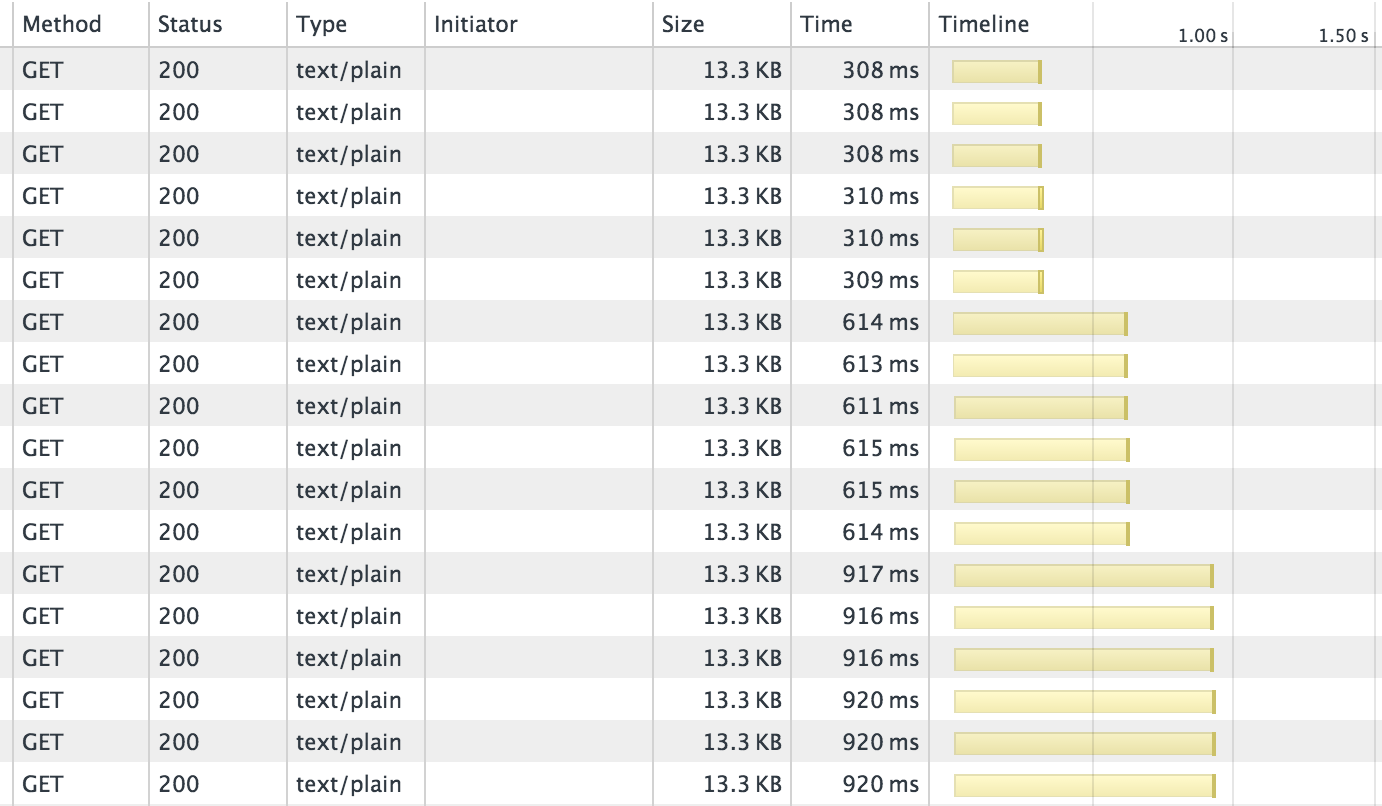
\includegraphics[width=0.9\textwidth]{images/chrome_latency_limit.png}
    \end{center}
  \caption{Chrome developer tools showing how the six TCP connection limit becomes a bottle neck on a connection with ~300 ms of latency.}
  \label{fig:tcp_bottleneck}
\end{figure}

We can calculate the total delay caused by latency in our example by with the following formula:

\begin{equation}
\mbox{total latency} = \mbox{number of thumbnails} * \frac{\mbox{latency per request}}{\mbox{number of parallel requests}}
\end{equation}

In our example, we fetch 60 thumbnails on a connection which has a latency of ~300 ms to the server. Our browser (Google Chrome) can handle six parallel TCP connections which gives us the following result:

\begin{equation}
\mbox{total latency} = 60 * \frac{300}{6} = 3,000 \mbox{ms} = 3 \mbox{seconds}
\end{equation}

If we instead could concatenate these 60 thumbnail-requests into one request, and the response instead would contain all of the thumbnails --- then we would only have to pay the latency cost once. This would reduce the total latency by an order of magnitude, from 3,000 ms to 300 ms, since we only have to pay the price for the latency once.

It is worth pointing out that increasing the bandwidth of the connection would not resolve this problem as the latency is the only bottleneck in this example.

It is not uncommon for browsers to wait idle for 100 - 150 ms before spending 5 ms to download an image. This means that latency is often accounting for 90-95\% of the total waiting time for the HTTP requests\cite{latency}.

\subsection{Chunked responses}
In the previous example where we fetched thumbnails, we often want to display them as soon as each individual image has been loaded and not wait for the entire concatenated response. 

When using a concatenated request to fetch multiple resources at the same time, the server can use chunked transfer encoding in the HTTP response to send the individual thumbnail data in chunks\cite{chunked}. By doing so, images, or any other data, can be displayed on the client as soon as each chunk is available, even out of order if necessary. 

This approach, with concatenated requests and a chunked response, has been successfully been implemented at Dropbox on their gallery software implementation\cite{dropbox_chunked}.

\section{Compression}
\label{compression}

All requested uncompressed data, such as text, can be compressed before it is sent to the client to reduce the transfered data size. A common compression algorithm used in HTTP requests is GNU Zip (Gzip) and works best on text-based files such as HTML, CSS and JavaScript. Gzip has an expected compression rate of 60-80\% when used on text-based files\cite[page 237]{HPBN}.

It is worth mentioning that there are scenarios where Gzip compression applied to very small files can increase the total size because of the Gzip dictionary overhead. This problem can be mitigated by defining a minimum file size threshold\cite{google_gzip}.

As an example, arbitrary user data for 50 users was created and stored in JSON format. When this data was requested from a server without compression, the total content-length of the HTTP request payload amounted to 55,205 bytes of data. By applying Gzip compression to the same data, the content length was reduced to 16,563 bytes of data which amounts to a 70\% space saving. 

\begin{equation}
\mbox{Space Saving} = 1 - \frac{\mbox{Compressed Size}}{\mbox{Uncompressed Size}} = 1 - \frac{16,563}{55,205} = 70\%
\end{equation}

An important thing to note about Gzip compression is that only the payload is compressed in HTTP/1.1\cite{header_compression}. This means that the headers, including cookies, are not compressed which would've otherwise been an additional performance gain. This is one of the improvements which have been addressed in the development of HTTP/2\cite[page 222]{HPBN}.

\chapter{API Gateways in theory}
When developing clients for a back-end API, you often find that the clients needs and the back-end APIs functionality isn't a perfect match. Different functionality is often required based on whether the client is a mobile application, a desktop application or something entirely different. The way the clients want to use the API can also radically differ based on what kind of product is being developed.

Not being able to optimise the API for each clients needs can hurt the clients performance since it has to do a lot of extra work but can also strain the developer whom may have to do extra work to refit the API for the clients.

Changing the back-end API is often not possible, especially in an enterprise environment. The back-end can be a legacy system which is not allowed to changed, it might be impractical to adapt the back-end for different client type without breaking existing clients or the back-end development team might be strained for any other reason.

One approach to solve this problem is by utilising an API gateway.

\section{What is an API Gateway?}
An API gateway works as an additional layer between the client and the server. For an API gateway to be efficient, it has to be able to augment the communication between the client and the server, and by doing so, improve the clients performance and implementation of the API.

It is also possible for an API-gateway to work in reverse and translate the clients requests for the server instead. This type of API-gateway is however not studied in this document.

\begin{figure}[H]
  \centering
    \begin{center}
      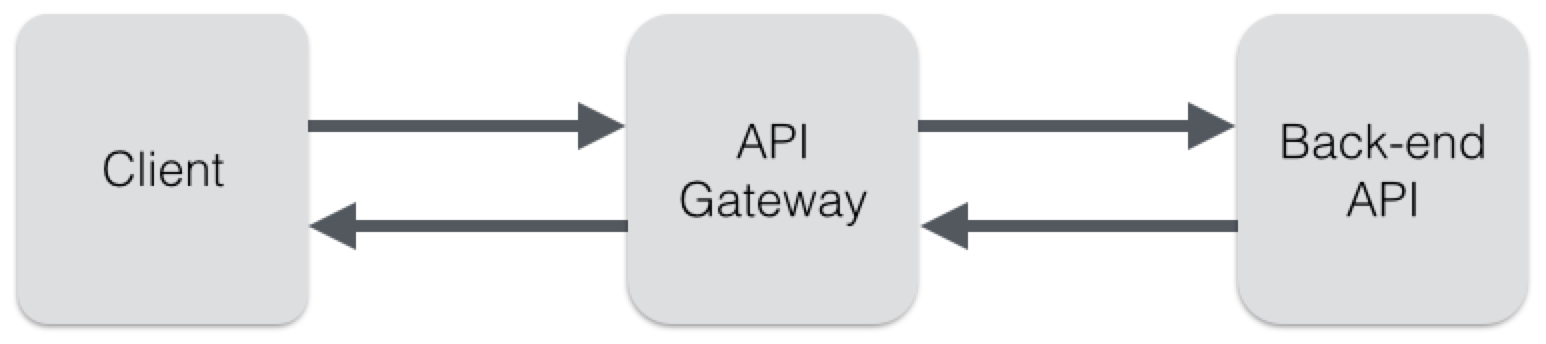
\includegraphics[width=0.9\textwidth]{images/api_gateway.png}
    \end{center}
  \caption{The API gateway is placed as a layer between a client and a back-end API.}
\end{figure}

\section{Differing client needs}
Nowadays, it is very common for different types of clients to consume the same API. One can imagine an image service with an API that returns a list of the latest uploaded images to some service. Depending on what type of client is requesting this data, the API gateway can augment the number of returned images. If the requesting device is a small mobile phone, the API gateway can chose to return a lot fewer images than if the requesting device was connected to a large wall monitor.

A similar approach has been implemented at Netflix where each client development team write their own adaptor code at the back-end to fully optimise the underlying API for that clients specific needs\cite{netflix}. This concept is much like in the same fashion as how an API-gateway works.

\section{Multiple resources \& requests}
A client often has to perform many requests simultaneously, either to one or multiple back-end APIs. A typical scenarios is when a user loads a web application for the first time and the applications initial state and data has to be retrieved or when multiple connected resources has to be loaded.

\begin{figure}[H]
  \centering
    \begin{center}
      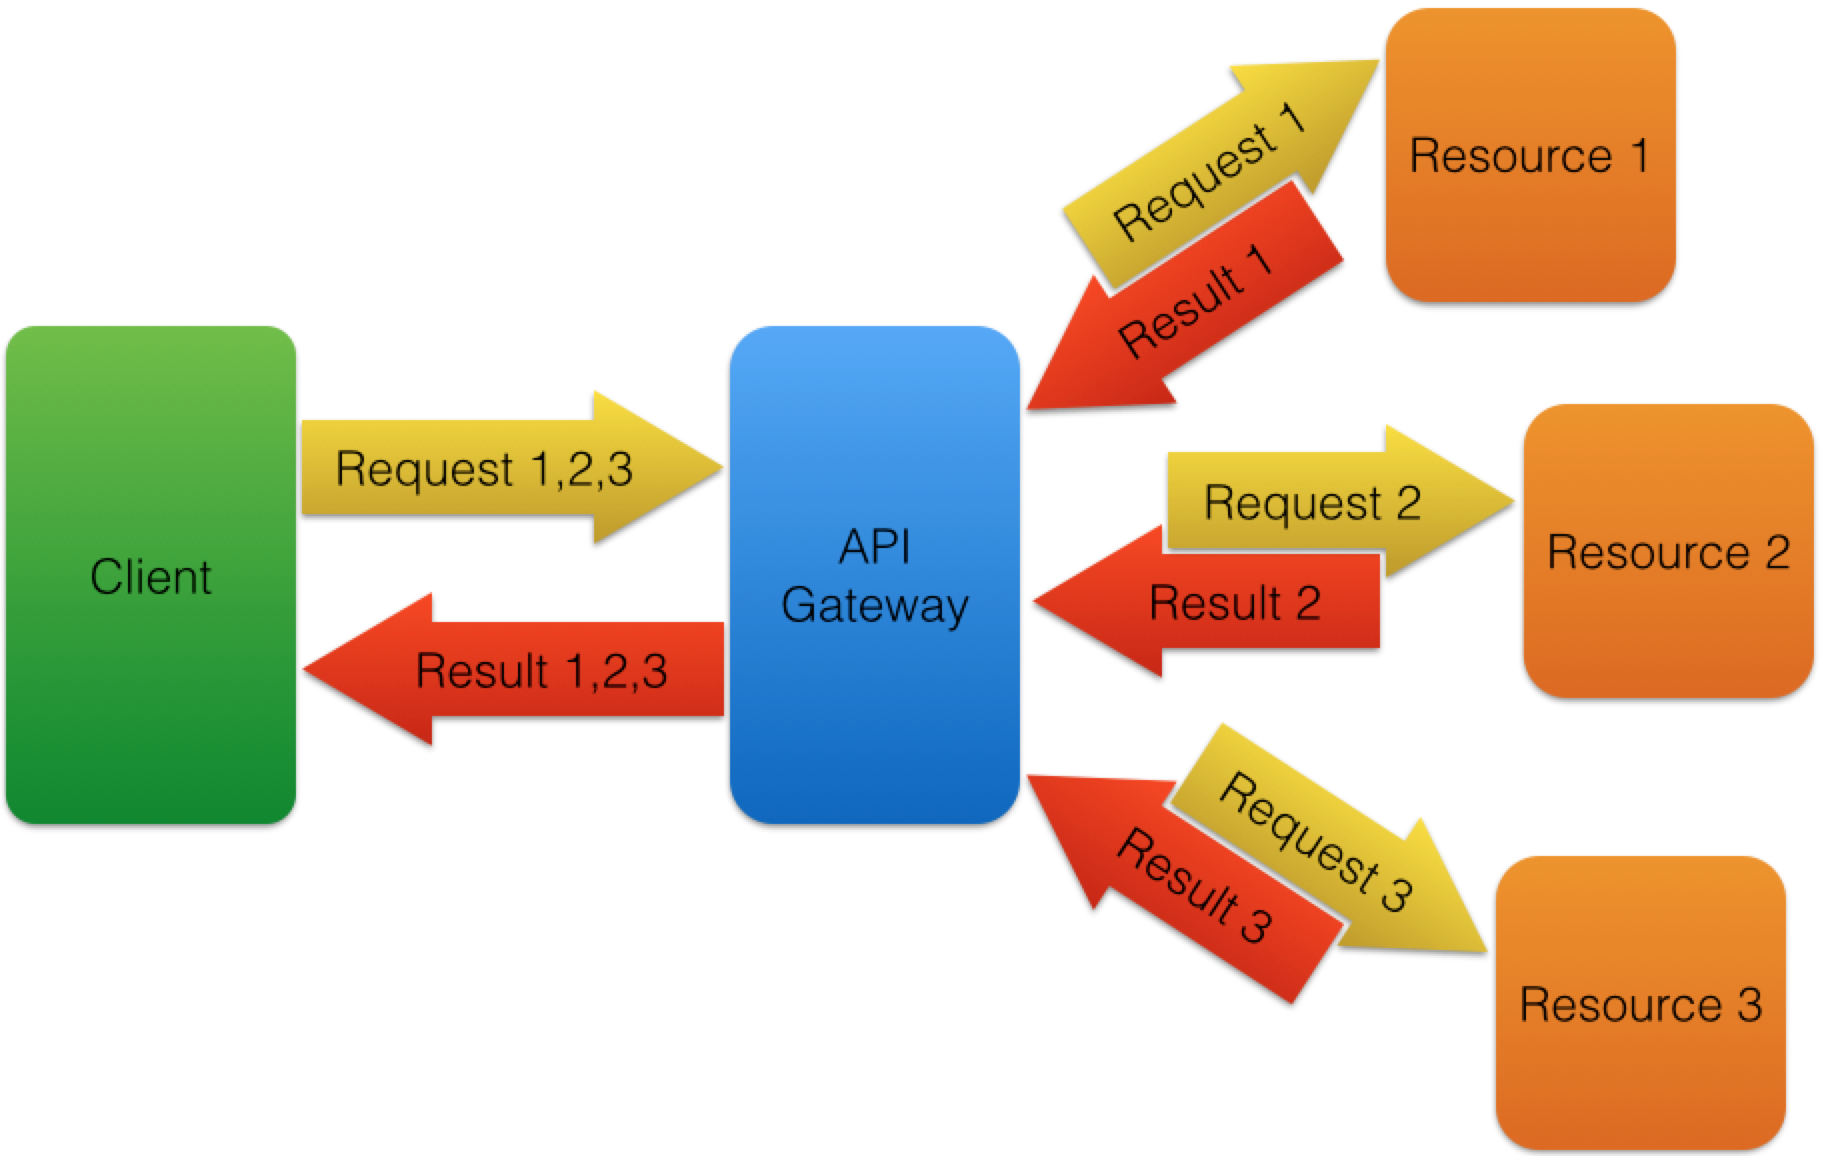
\includegraphics[width=0.9\textwidth]{images/api_gateway_concatenation.png}
    \end{center}
  \caption{An API gateway receives a concatenated request which it distributes to multiple resources, the responses are then concatenated into a single response. The resources can either belong to one or several back-end systems.}
\end{figure}

When working with HTTP requests, there are multiple penalties for executing many small requests compared to one concatenated request. These penalties includes the previously mentioned limit of maximum TCP connections (page \pageref{max_tcp}) and the overhead from http headers (page \pageref{headers}).

\section{Duplicate \& Unnecessary items}
When requesting data from a back-end API, the response may contain unnecessary data which the client doesn't need. In a similar fashion, if a client performs several similar requests, it is possible that all the responses contains some amount of duplicate data. By using an API gateway, the results from the back-end API can be augmented to remove those items that the individual clients does not need.

\begin{figure}[H]
  \centering
    \begin{center}
      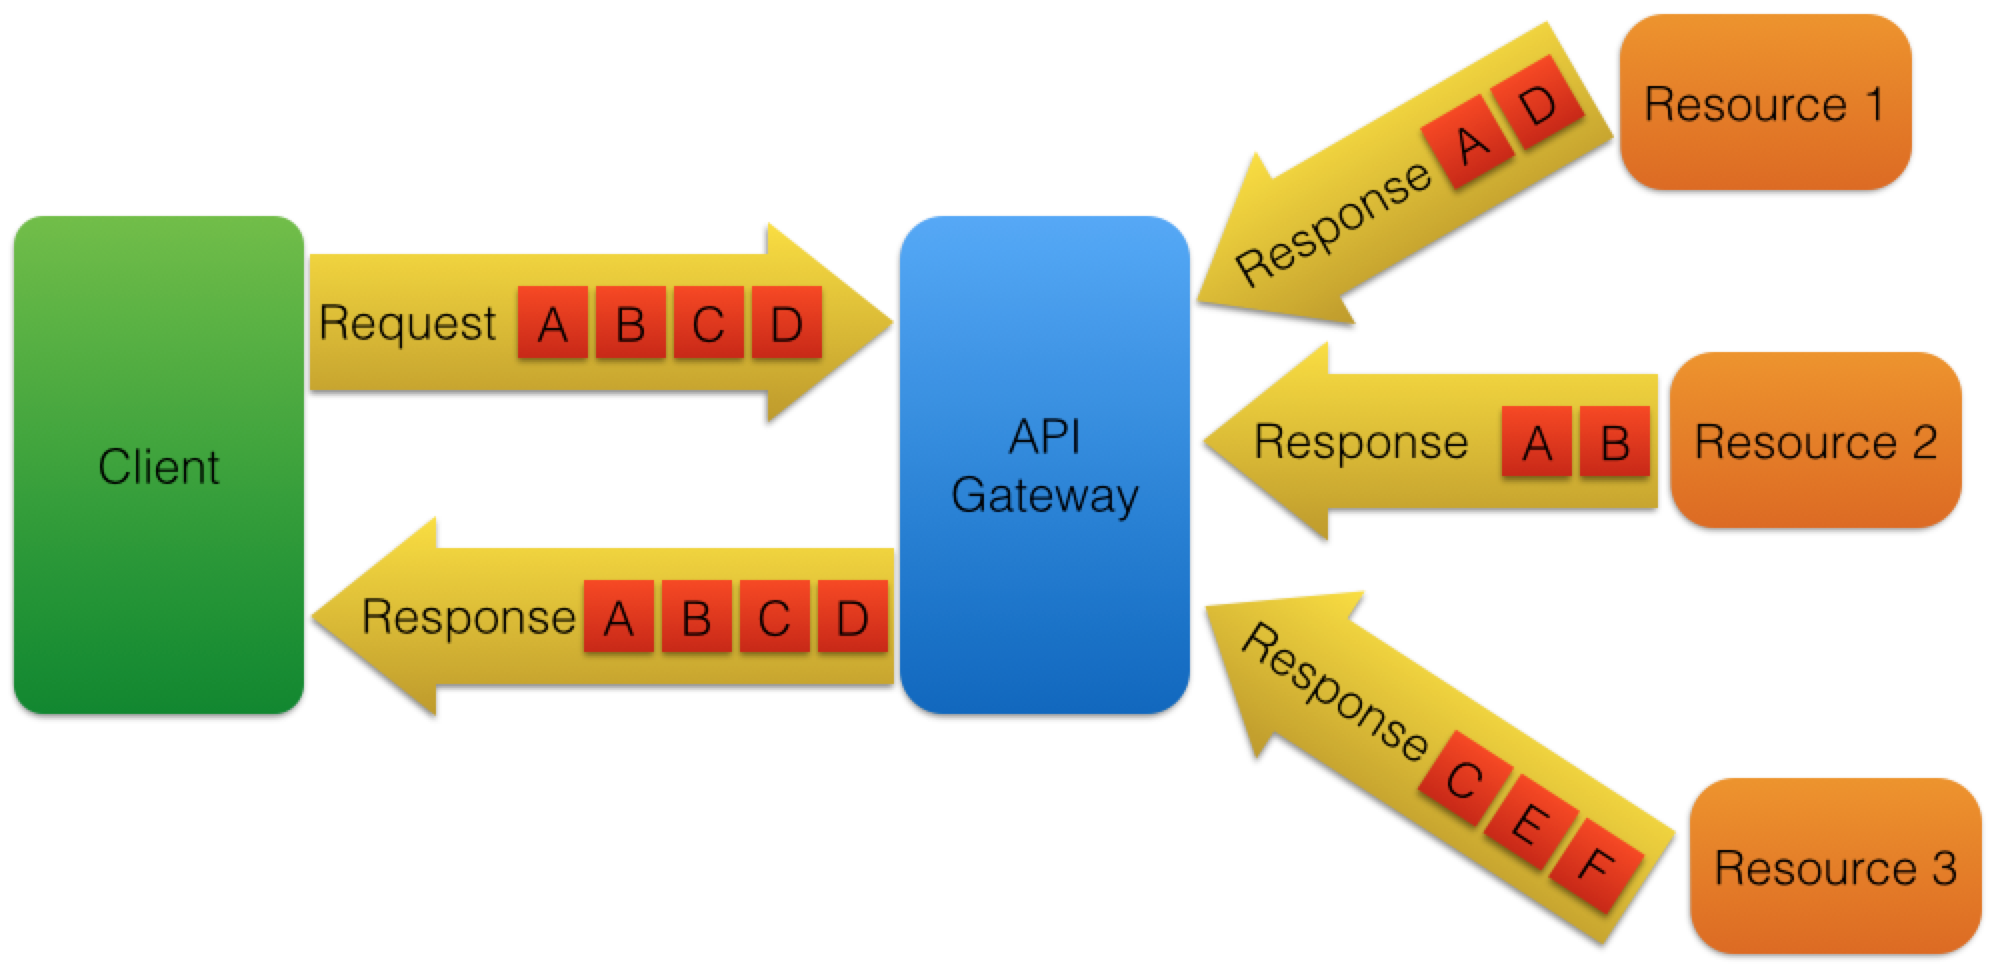
\includegraphics[width=0.9\textwidth]{images/api_gateway_duplicate.png}
    \end{center}
  \caption{The client request the items A, B, C, D. The API gateway fetches A, D from Resource 1. Item A from the Resource 2 response can be discarded since it's duplicate data. Item E, F from Resource 3 can be discarded since they are not wanted by the client. The API gateway can after retrieval respond with just the requested items A, B, C, D.}
\end{figure}

\section{Format transformation}
It is common when working with older legacy systems that the data is formatted in a way which is not suitable for modern clients. In the case of JavaScript, many browsers and developers prefer to work with JSON rather than XML. An API gateway can, on the fly, convert the data from the back-end to a format more appropriate for the requesting client and respond with it.

\begin{figure}[H]
  \centering
    \begin{center}
      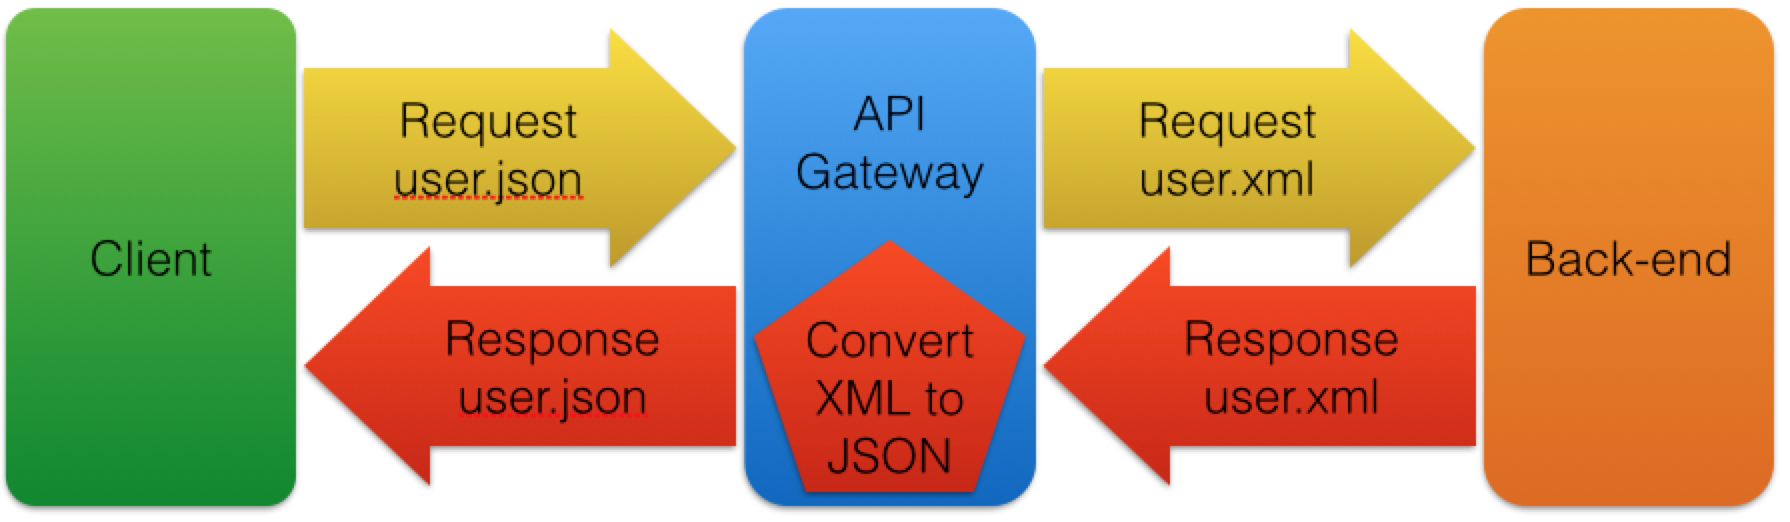
\includegraphics[width=0.9\textwidth]{images/api_gateway_transform.png}
    \end{center}
  \caption{The client requests "user" in JSON-format. The API gateway fetches "user" in XML-format from the back-end, converts it to JSON and responds to the client in the appropriate format.}
\end{figure}

This approach has the benefit that the conversion code does not have to be rewritten for every client. Rewriting the same conversion code, potentially in a new language, for each client increases the risk of introducing bugs related to the conversion because of the larger code bases\cite{code_complete}. 

By performing the transformation in the gateway, the processing work is moved away from the client which can improve its performance as well.

\section{Pure REST \& HATEOAS}
If an API follows the strict rules of REST, it utilises the concept of Hypermedia as the Engine of Application State (HATEOAS). Instead of defining a collection of end-points which the client can utilise, it requires the client to discover the resources itself by first performing a GET request to the APIs root. To root will respond with the resources available, such as users. The client then has to query the users root to discover which requests can be made in regards to the users resource --- and so on. Working in this way is very demanding for the developer which has to work with the API in the client\cite[page 61]{AASG}.

API-gateways can be used to transform a Pure REST API with HATEOAS to a simpler API which only follows some of the restrictions put in place by REST. This can significantly lower the amount of traffic between the client and the back-end, which can be a big performance gain in cases such when the latency is high between the client and the back-end --- assuming that the latency between the API gateway and the back-end is low such as when they are placed inside the same LAN.

\begin{figure}[H]
  \centering
    \begin{center}
      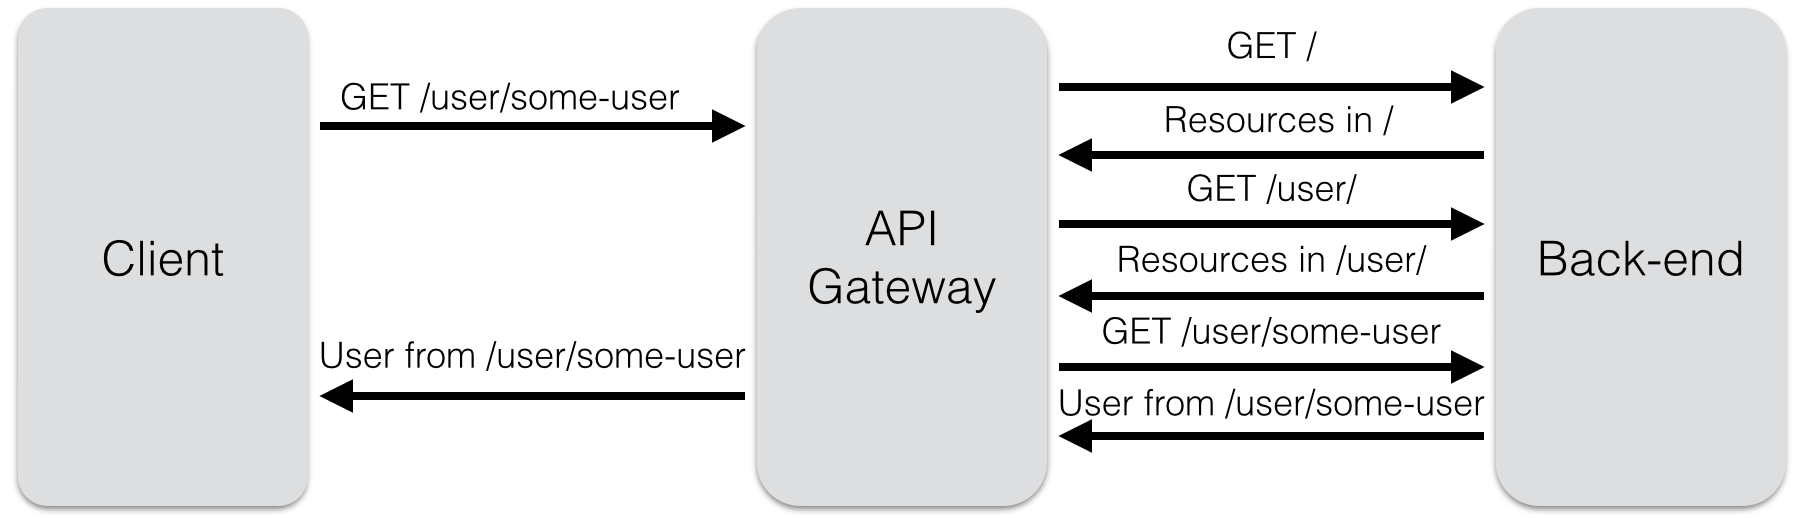
\includegraphics[width=0.9\textwidth]{images/api_gateway_hateoas.png}
    \end{center}
  \caption{Scenario where the API gateway performs the pure REST HATEOAS-communication and at the same time exposes a simple end-point for the client.}
\end{figure}

\section{Compression}
API gateways can be used to compress responses in the cases where no compression is present on the back-end API. This can significantly reduce the amount of traffic the client has to receive which increases the performance, especially on mobile devices. HTTP compression was explored on page \pageref{compression} where it was noted that Gzip has an expected compression level of 60-80\% on text-based media.

\begin{figure}[H]
  \centering
    \begin{center}
      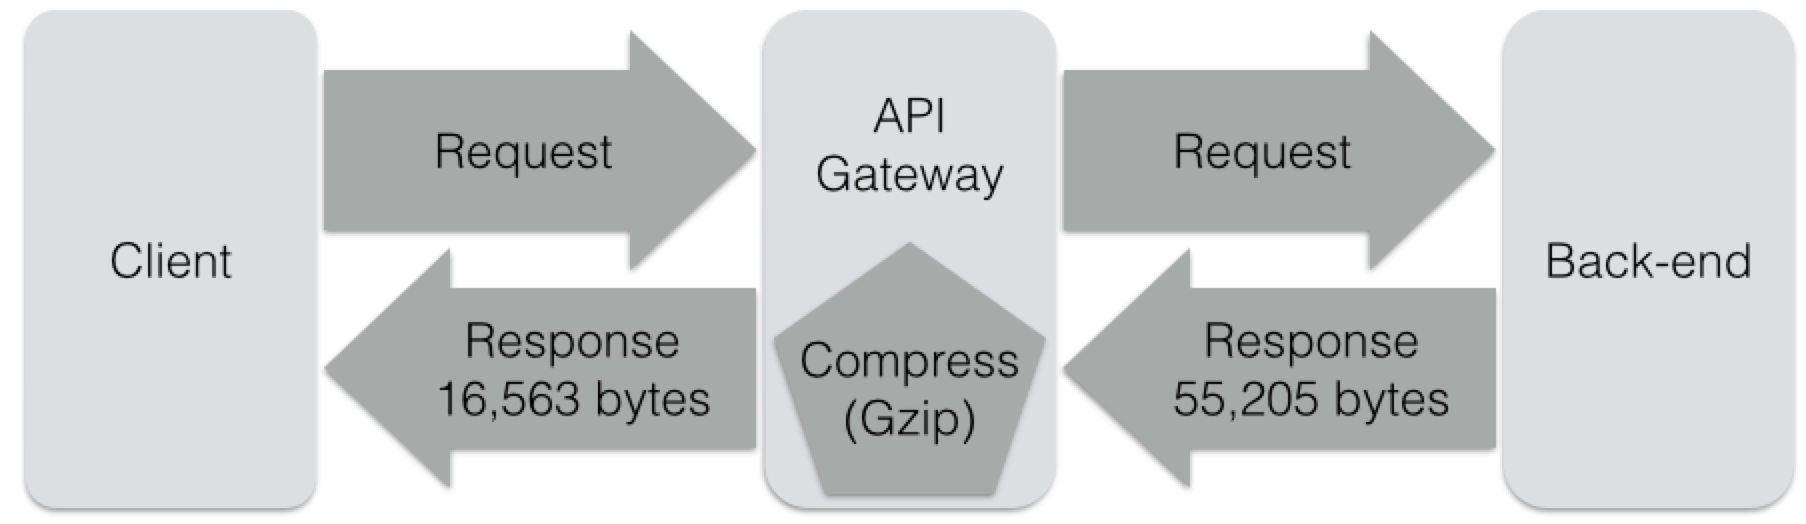
\includegraphics[width=0.9\textwidth]{images/api_gateway_compression.png}
    \end{center}
  \caption{The API gateway compresses the response from the back-end API with Gzip which reduces the response traffic in the client by 70\%. Numbers taken from the example on page \pageref{compression}.}
\end{figure}

\section{Caching}
Responses from frequent API calls can be cached using the API gateway to reduce the load on the back-end system\cite[page 107]{AASG}. The cache can have a specified lifetime or be invalidated based on certain events such as a table update on a database. There are several different caching strategies and third-party systems which the API-gateway can utilise --- this subject is a vast and complex topic in itself and is therefore not explored further in this document.

\begin{figure}[H]
  \centering
    \begin{center}
      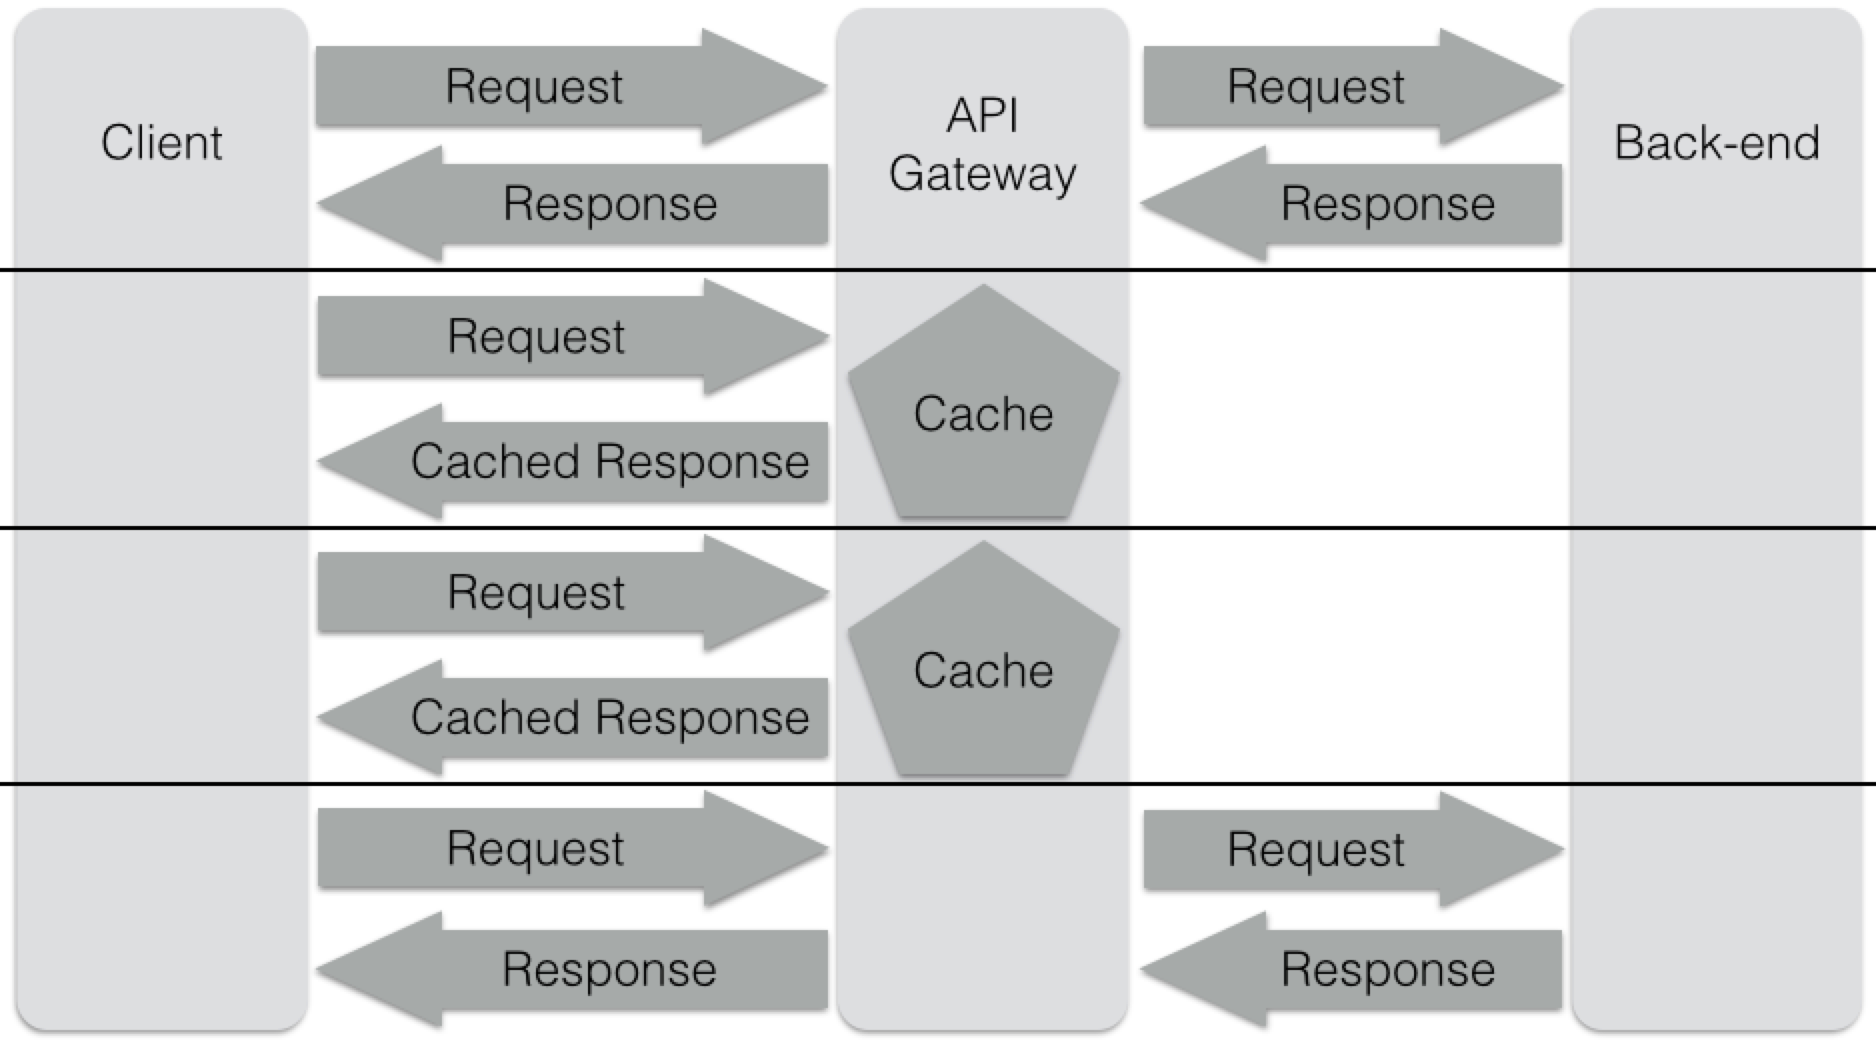
\includegraphics[width=0.9\textwidth]{images/api_gateway_cache.png}
    \end{center}
  \caption{Frequent API calls to the same end-point can be cached to reduce the load on the back-end.}
\end{figure}

\section{Decreasing bandwidth \& cost}
Cloud providers, such as Amazon\cite{cloud_amazon} and Microsoft\cite{cloud_microsoft}, do not charge for the bandwidth as long as data is transfered between servers in the same cloud regions. When using an API-gateway in the cloud, bandwidth \& its costs can be reduced by placing the API-gateway in the same cloud region as the back-ends and apply bandwidth saving techniques such as the previously in this chapter mentioned: compression, duplicate \& unnecessary items, pure REST and in some cases even format transformation.

\begin{figure}[H]
  \centering
    \begin{center}
      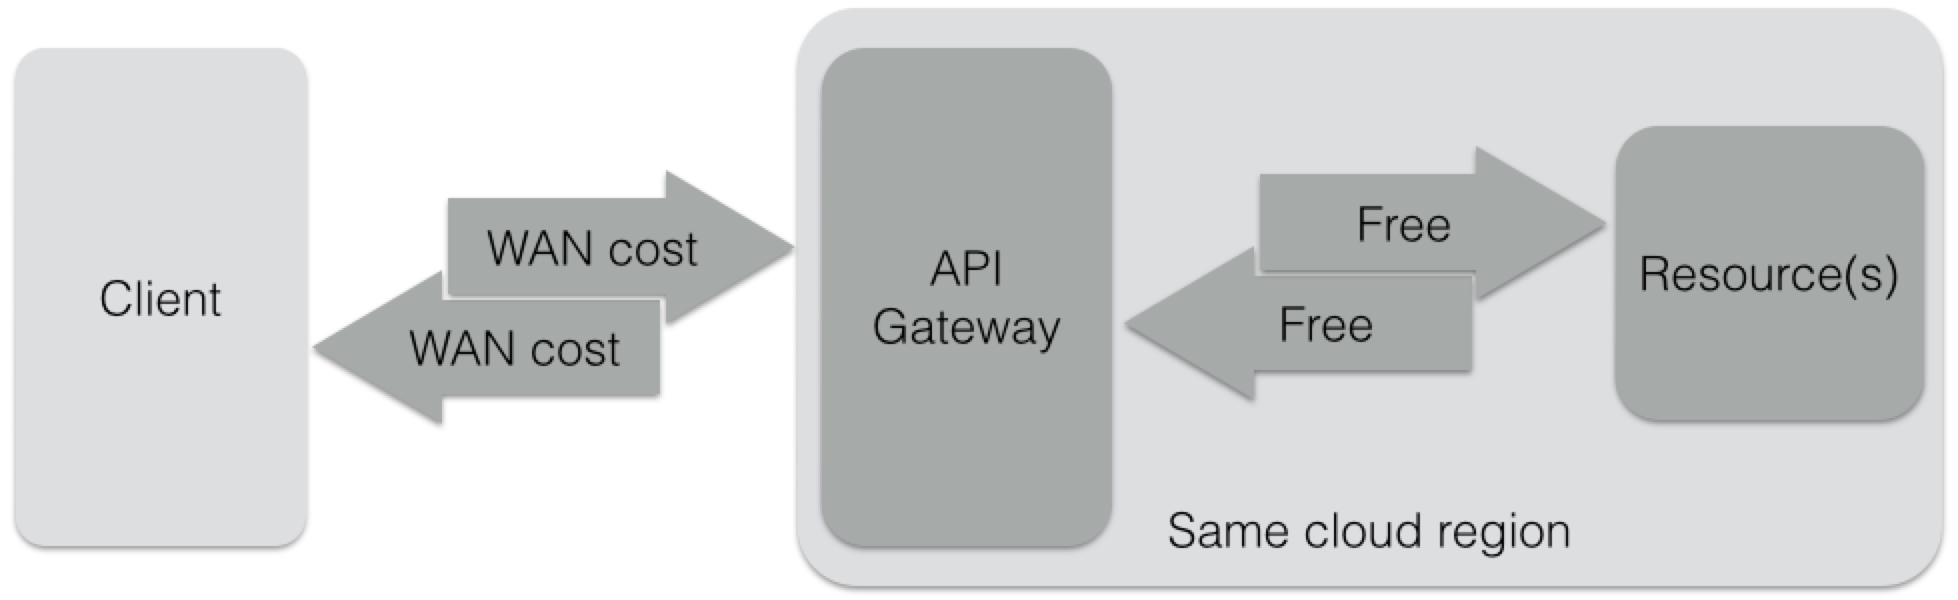
\includegraphics[width=0.9\textwidth]{images/api_gateway_bandwidth.png}
    \end{center}
  \caption{Cloud providers such as Amazon\cite{cloud_amazon} and Microsoft\cite{cloud_microsoft} charges based if the traffic is over WAN or in the same cloud region.}
\end{figure}

\section{Secure point of entry for private networks}
It is not uncommon for corporations to have several internal services with APIs which are protected inside a private network. A VPN, virtual private network, can be utilised to give clients on the outside access to services inside the private network. A VPN can however have the side effect of exposing to much of the private network to the client machines.

Another approach is to place an API-gateway inside the DMZ of the private network. By doing so, outside clients can access the API-gateway as a single point of entry for all internal APIs. The API-gateway can be configured to expose a defined collection of the internal APIs and proxy them to the outside clients.

\begin{figure}[H]
  \centering
    \begin{center}
      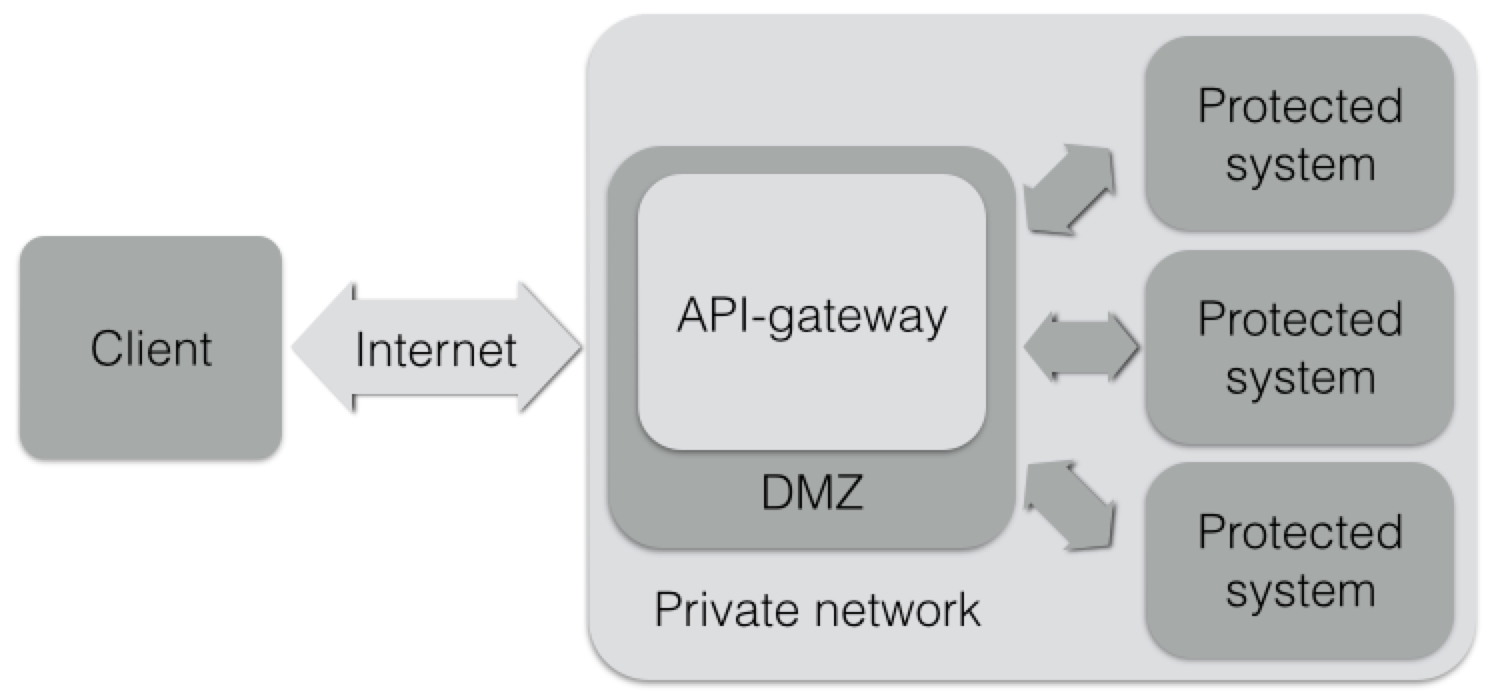
\includegraphics[width=0.9\textwidth]{images/api_gateway_dmz.png}
    \end{center}
  \caption{An API-gateway used as a secure way of exposing internal services in a private network to the outside world.}
\end{figure}

\section{Latency}
One important goal of an API-gateway is to reduce, or at least not increase, the latency in the communication between the client and the back-end. Because of this, the placement of the API-gateway, from a network point of view, is very important. 

The first approach is to place the gateway on the same LAN or together with the client. Placing the API-gateway on the same machine as the client is rarely possible or practical. It complicates updating the gateway and defeats much its purpose. 

Placing the API-gateway inside the same LAN as the client can be a good solution, for example when used inside corporation. The constraint with this approach is that no outside clients, such as smartphones not connected to the LAN, will be able to avoid the extra latency introduced over WAN --- or may not be able to connect to it at all based on the LAN security. This is however an approach which does not introduce double latency.

The second approach is to place the API-gateway as a separate application in its own cloud or on a LAN separated from the backend. While this may be the only solution for certain hosting setups, this introduces the problem of double latency. Since the TCP-packets has to go through two WAN connections, both of them can introduce a substantial amount of latency which can worsen the response time.

Finally, the third approach is to place the API-gateway on the same LAN as the back-end system. This is in many cases the best approach as it avoids the double latency, gives access to outside clients and introduces flexibility in regards to updates. 

The problem with double latency can however arise and be unavoidable if the API-gateway is communicating with several back-end systems which are placed on different LANs. In such a scenario, several factors have to be considered before deciding which LAN to place the gateway in such as the which back-end API has the most traffic, bandwidth costs between LANs, the latency between the different LANs and so on.

\begin{figure}[H]
  \centering
    \begin{center}
      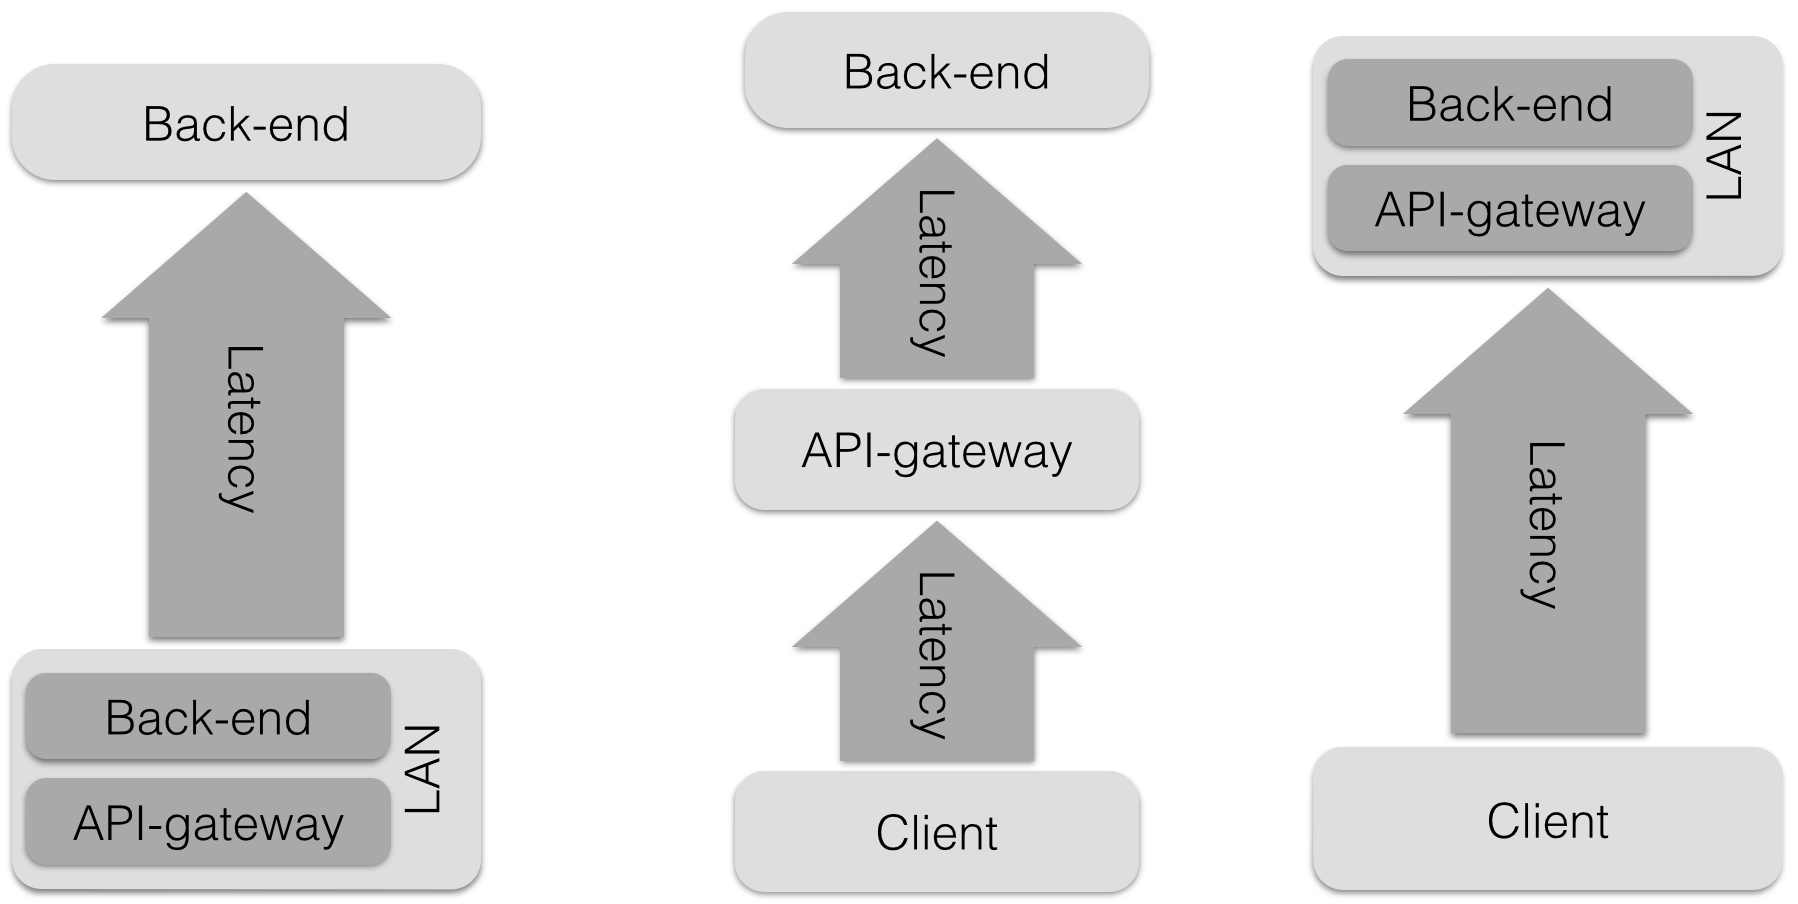
\includegraphics[width=0.9\textwidth]{images/api_gateway_latency.png}
    \end{center}
  \caption{How latency affect the different placement strategies for the API-gateway.}
\end{figure}

\section{Security - authentication \& authorisation}
\label{sec:security}
API-gateway security is, like all security scenarios, a complex issue. All but the simplest cases should be solved outside the implementation of the gateway itself. What makes an API-gateway complex from a security point of view is the fact that one end-point provided from the API-gateway can communicate with several back-end systems, all of which can utilise different authentication and authorisation protocols. Because of this, a single sign-on service provided outside the API-gateway itself is a good approach for the more complex API-gateways which integrate with several back-end systems.

Further in-depth discussion around this topic is outside the scope of this document

\section{Old API version support}

It happens that API developers makes changes which breaks backward compatibility when moving on to newer versions. Fields can be added, renamed or removed. In such scenarios, old clients may be forced to update in order to work with these breaking API changes.

Instead of rewriting many of the already released clients to fit the new API-version, an API-gateway can, in some cases, be used to translate the new API format to the old one. How feasible this is depends on what kind of changes has been introduced and whether they are destructive or not.

\section{Analytics}

API-gateways are in a perfect position to collect data to be used for analytics since the API-gateway is able to monitor all traffic between the clients and the back-ends. 

An API-gateway can easily collect analytics from HTTP data such as:
\begin{itemize}
	\item Client technology, the browsers user-agent which is sent with request headers is one way to collect a variety of data. Example: User-Agent: Mozilla/5.0 (Macintosh; Intel Mac OS X 10.10; rv:37.0) Gecko/20100101 Firefox/37.0.
	\item Request-response time for both the client and individual back-end APIs.
	\item Latency from different back-end APIs.
	\item Geolocation from HTML 5 geolocation API\cite{html5_geolocation} or by geolocating the requesting IP address.
	\item Errors from back-end APIs.
	\item Invalid client requests.
	\item Traffic peak hours.
	\item Suspicious client behaviour such password or denial of service attacks.
\end{itemize}

Since performance is a top priority in API-gateways, the collected data should preferably be delegated to and stored and processed using a third-party analytics engine.

\chapter{Crocodile Pear: API-gateway framework}

\section{Language \& Libraries}
\subsection{Elixir}
Elixir is a functional language designed for building scalable and maintainable applications on the Erlang Virtual Machine. The Erlang VM is known for running low-latency, distributed and fault-tolerant systems while also being successfully used in web development\cite{elixir}. Properties all of which are important for a successful API-gateway implementation.

Two other important influences for choosing Elixir in this prototype are the pipe operator and the asynchronicity achieved by utilising Elixir processes.

\subsection{The pipe operator}
One of the integral parts of Elixir is the pipe operator: $|>$. The pipe operator takes the output from the expression left side of the operator and pipes it into the first argument of the right hand side function. People who are accustomed to Unix may see the similarity with the Unix pipe operator: $|$.

As an example, we can take a look at the following nested and hard to read code:

\begin{figure}[H]
  \centering
\begin{lstlisting}[breaklines=true,frame=single]
Enum.sum(Enum.filter(Enum.map(1..100_000, &(&1 * 3)), odd?))
\end{lstlisting}
  \caption{Elixir code written without the pipe operator.}
\end{figure}

The code from the figure above can be rewritten using the pipe operator which results in a more easily read version:

\begin{figure}[H]
  \centering
\begin{lstlisting}[breaklines=true,frame=single]
1..100_000 |> Stream.map(&(&1 * 3)) |> Stream.filter(odd?) |> Enum.sum
\end{lstlisting}
  \caption{The same code as in the previous figure but written with the pipe operator.}
\end{figure}

This also has the good side-effect that ti makes you reason about the code in a better way. When you read it, you might say something like: "First I have the range of numbers, then I map over it, then I filter them, then I sum them".

The pipe operator is an important part in how Crocodile Pear works, as it pipes requests to a result, potentially through transformations along the way. This makes CrocodilePear's syntax look like an easy to read DSL (Domain Specific Language) for exposing endpoints and piping requests to the client.

\subsection{Elixir processes}
Processes are Elixir's term for utilising the Actors model as its concurrency model. In Elixir, processes are extremely lightweight (compared to operating system processes) which means that it is not uncommon to have thousands of them running simultaneously. Elixir processes run concurrently, isolated from each other and can only communicate by message passing\cite{elixir_processes}.

\subsection{Plug}
Plug is a specification for composable modules in between web applications - and works as connection adapters for different web servers in the Erlang VM\cite{plug}. In Crocodile Pear, Plug is utilised for exposing end-points to the clients to which they can send requests, and a way for the API-gateway to send responses back over HTTP to the clients.

\subsection{HTTPoison}
Internally, Crocodile Pear uses HTTPoison\cite{httpoison}. It is based on hackney\cite{hackney}, and it is used to send HTTP requests to back-end systems. The HTTPoison library is only used internally and is therefore abstracted away to simplify the API-gateway development and ensure that it can be removed or replaced in the future.

\section{High-level concept}

\subsection{Data}
The data used in Crocodile Pear corresponds to that of an HTTP request. It consists of a numeric HTTP code, such as 200 for OK, headers which is an key-value map and an arbitrary amount of chunks which makes up the actual data payload of the HTTP request/response, in this document called the body - not to be confused with the HTML body-tag. 

In addition to this, a meta-data map is available for storing data outside the HTTP-model. This can be utilised to pass intermediate meta-data between requests which are not part of the requests themselves.

\subsection{Processes: producers \& consumers}
The key component in Crocodile Pear's asynchronous behaviour is the relationship between producers and consumers. Both consumers and producers are fully asynchronous Elixir processes which communicate by passing messages between each other. When a consumer is ready to receive data from a producer, it sends a message to the producer with its identity and a status telling the producer that it is ready to receive.

\begin{figure}[H]
  \centering
\begin{lstlisting}[breaklines=true,frame=single]
send(producer, { self, :ready })	
\end{lstlisting}
  \caption{The consumer sends a tuple with status "ready" and the identity of itself, using the function self(), to the producer when it is ready to receive data.}
\end{figure}

The identity of the producer is always known to the consumer via an Elixir PID, process identification, which is passed around in the pipeline (explained below). The producer will only produce a response once and will terminate after a consumer has consumed the response.

\begin{figure}[H]
  \centering
    \begin{center}
      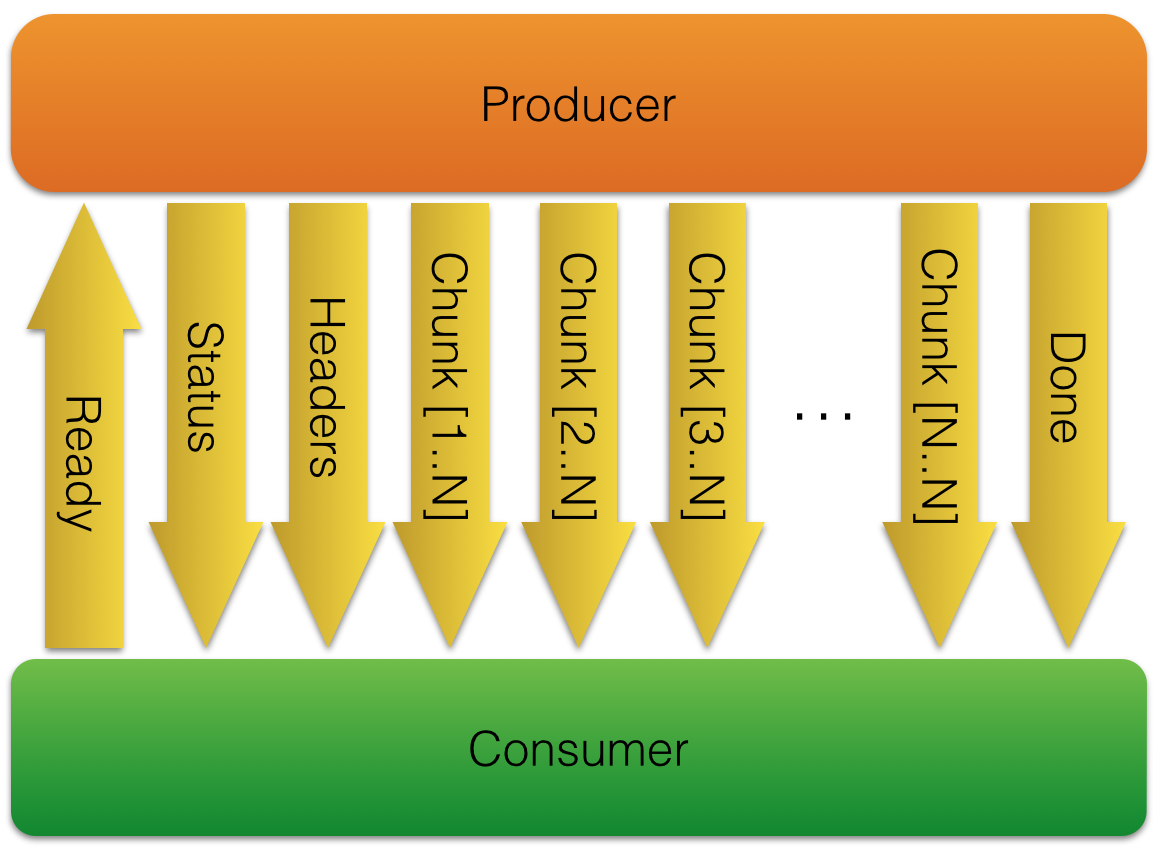
\includegraphics[width=0.9\textwidth]{images/crocpear_producer_consumer.png}
    \end{center}
  \caption{Message passing between a producer and a consumer. Time flows from left to right.}
\end{figure}

After the producer has been notified that a consumer is ready to consume its data, it must first respond with the status, the headers and the meta data. After that, the chunks must be sent in order. Finally, a done message is sent indicating that the producer will terminate and all chunks have been sent.

All Elixir processes, the consumers and producers, are abstracted away from the end-user of the framework. Instead, the end-user only works with functions which are applied to all chunks combined on a per request basis. Abstracting away the concurrency model has in practice no performance penalty while it does makes the development a whole lot easier. There is, however, nothing that hinders a developer to work on the lower process level if that for some reason is wanted.

\section{Pipeline}
The pipeline is what ties all pieces in Crocodile Pear together. The pipeline follows a simple rule: every intermediate function in the pipeline should take a list of producer PIDs as its first argument and return a new list of producer PIDs as its only return value.

The two exceptions are the functions $request$ and $response$ which normally are the beginning and the end of each pipeline. It is also possible to mix a CrocodilePear pipeline with a normal function pipeline in Elixir, this is explored further in the examples below.

\subsection{Request}
The $request$ function in Crocodile Pear takes an arbitrary number of URLs as strings or a map structure if more advanced settings is needed such as specifying request headers, the HTTP method GET, POST and so on. The $request$ will always return a list of producer PIDs. Each producer will produce the response from one HTTP request from the specified URL.

\subsection{Response}
The $response$ function takes a list of producers and turns them in to an HTTP response by utilising the provided $conn$ in $Plug$. If more than one producer is passed to the $response$ function, the first responding producer will be consumed first which means that the response order is not deterministic --- if not explicitly defined so. However, the first responding producer will be consumed fully before any other producer is consumed which guarantees that the chunks will not be mixed together.

As soon as one of the chunks from a producer has been consumed by the response function, it will respond to the client with it by utilising the chunked HTTP response.

\subsection{Transformers}
Transformers are a concept used in CrocodilePear to manipulate the response data form a request while it flows through the pipeline without exposing the underlying concurrency model.

The transformer function takes a lambda function as its only parameter. This lambda is called with the response map, as soon as its available, as its only parameter and allows transformations to take place.

\begin{figure}[H]
  \centering
\begin{lstlisting}[breaklines=true,frame=single]
blanker = fn(response) ->
  response
  |> Dict.update!(:status, fn(_discarded_status) -> 404 end)
  |> Dict.update!(:headers, fn(_discarded_headers) -> %{} end)
  |> Dict.update!(:body, fn(_discarded_body) -> "" end)
  |> Dict.update!(:meta, fn(_discarded_meta) -> %{} end)
end
\end{lstlisting}
  \caption{The function blanker is a simple lambda function which can be used in a transformer. It sets the status to 404 and removes all headers, the meta-data and the payload by simply ignoring the received values and providing corresponding empty values instead. The actual data in status, headers and body are discarded by using an underscore at the start of the function call in Dict.update!.}
\end{figure}

\subsection{Timers}
Crocodile Pear include timers which can be placed anywhere in the pipeline to benchmark the time it takes to reach the different stages. Timers can be used anonymously or with labels attached to them and they will output data to the default logger. The timers also work with the underlying concurrency model which means that every single chunk in from any of the processes can be timed individually.

\begin{figure}[H]
  \centering
\begin{lstlisting}[breaklines=true,frame=single]
10:41:57.437 [info]  {1424, 252517, 434960} (Got URL)
10:41:58.187 [info]  {1424, 252518, 187494} [headers] (Executed request) on #PID<0.256.0>
10:41:58.187 [info]  {1424, 252518, 187591} [status] (Executed request) on #PID<0.256.0>
10:41:58.187 [info]  {1424, 252518, 187728} [chunk] (Executed request) on #PID<0.256.0>

[...]

10:41:59.529 [info]  {1424, 252519, 529096} [status] (Added transform function) on #PID<0.431.0>
10:41:59.529 [info]  {1424, 252519, 529177} [headers] (Added transform function) on #PID<0.431.0>
10:41:59.543 [info]  {1424, 252519, 543830} [chunk] (Added transform function) on #PID<0.431.0>
10:41:59.544 [info]  {1424, 252519, 543943} [done] (Added transform function) on #PID<0.431.0>
10:41:59.544 [info]  {1424, 252519, 544106} (Responded to query)
\end{lstlisting}
  \caption{The output from the logger. From left to right: time when message is logged, log level, Erlang timestamp \{MegaSecs, Secs, Microsecs\}, [message atom] optional message (producer PID if present).}
\end{figure}

\subsection{Concatenate JSON}
The function $concatenate\_json$ takes a list of producers, consumes them and returns a new producer. The new producer's chunks will be the responses from the previous consumers, concatenated to a JSON list. Each chunk sent by the new producer will be one item from the JSON list, along with some JSON syntactical data. The order is determined based on which producer starts responding first.

Each item in the list will be a JSON-object containing the four keys: status, headers, meta and body (payload). Optionally, if a "true" value is passed in to the function, each item in the list will be only the "body" (payload) with the headers, meta and status omitted.


\begin{figure}[H]
  \centering
    \begin{center}
      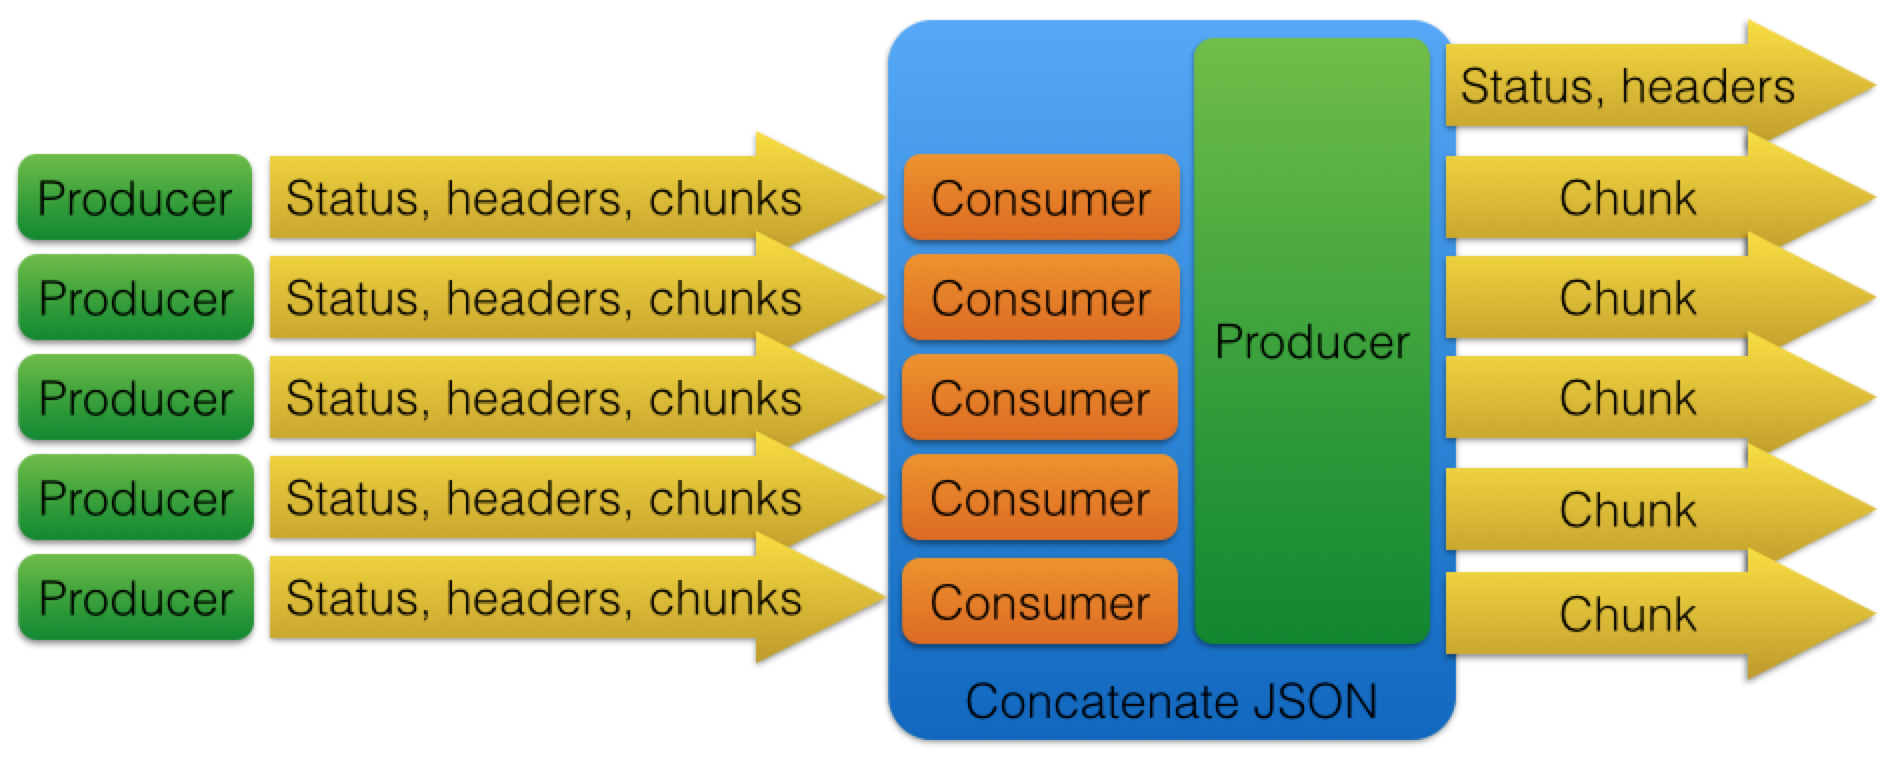
\includegraphics[width=0.9\textwidth]{images/crocpear_concatenate_json.png}
    \end{center}
  \caption{Concatenate JSON creates one consumer for each producer. As soon as one consumer has consumed an entire response, the new producer will send that as a chunk in JSON format.}
\end{figure}

Even though $concatenate\_json$ takes an arbitrary number of producer PIDs as its argument, it will itself only return one new producer as its result is one JSON list object.

\subsection{Creating end-points}
todo...

\section{Examples}
\subsection{Request proxying}
A simple proxy is a good introduction example which demonstrates how the request / response pipeline can be used. In this example, we extract an URI from the query string in the connection and pipe it to the $request$ function which in turn is piped into the $response$ function.

\begin{figure}[H]
  \centering
\begin{lstlisting}[breaklines=true,frame=single]
conn.query_string
|> request
|> response(conn)
\end{lstlisting}
  \caption{A simple proxy.}
\end{figure}

In a similar fashion, we could take an arbitrary number of requests and proxy them into one result. Here we take several URIs from the query string, separated by the character "|" and pipe them in to the $request$ and $response$ functions as before. By using Elixirs String.split, a list of strings is created which is passed into the $request$ function.

\begin{figure}[H]
  \centering
\begin{lstlisting}[breaklines=true,frame=single]
String.split(conn.query_string, "|")
|> request
|> response(conn)
\end{lstlisting}
  \caption{A simple proxy for an arbitrary number of URIs.}
\end{figure}

This will execute all requests concurrently and start responding, in indeterministic order, based on which of the requests is responding first.

\subsection{Concatenate responses to JSON}
The concatenate\_json function can be used to concatenate several requests into a JSON list object. It will also set the "Content-Type" header to the appropriate "application/json".

\begin{figure}[H]
  \centering
\begin{lstlisting}[breaklines=true,frame=single]
String.split(conn.query_string, "|")
|> request
|> concatenate_json
|> response(conn)
\end{lstlisting}
  \caption{Demonstration of the concatenate\_json function.}
\end{figure}

The response will be one JSON list where each item  in the list contains the response's status, headers, meta and payload as an JSON objects.

\subsection{Transformers}
In this more complex example, we will use all previously explained techniques along with a transformer to create a more powerful end-point. We will go over the code in the following figure line by line.

\begin{figure}[H]
  \centering
\begin{lstlisting}[breaklines=true,frame=single]
get "/temperature" do
  uris =
    String.split(conn.query_string, "|")
    |> Enum.map(&("http://api.openweathermap.org/data/2.5/weather?q=#{&1}"))

  temperature_extractor = fn(item) ->
    Dict.update!(item, :body, fn(body) ->
      response_body = Poison.decode!(body)

      Map.put(%{}, response_body["name"], response_body["main"]["temp"])
      |> Poison.encode!
    end)
  end

  uris
  |> request
  |> transform(temperature_extractor)
  |> concatenate_json(true)
  |> response(conn)
end
\end{lstlisting}
  \caption{A complex example with a transformer.}
\end{figure}

On line 1, we expose the new end-point /temperature from the API-gateway on which we'll wait for GET requests.

On line 2 - 4, we intercept cities and country codes, such as "Lund,SE|Copenhagen,DK", from the query string sent through the connection and then split them in to a list using the separating character: $|$. This list is then mapped over which will create the appropriate URLs to call for the underlying API which we will use in this example.

On line 6 - 13, we create a new transformer lambda function. When we receive the actual payload data, the body, we will decode it from JSON format to native Elixir data types using the third-party library Poison\cite{poison}. We will create a new JSON object by extracting the name and temperature as a new key-value pair and encode it using Poison again - the rest of the payload data is discarded. The other response data: status, headers and meta, will be left intact since our function only updates the data stored within they key :body.

On line 15 - 19, we tie everything together using the pipeline. We take the URIs, pipe them into a request, pipe the request in to a transformer with our new function $temperature_extractor$, pipe that in to the concatenate\_json function and pipe that to the response.

In this example, we have used request/response concatenation, discarding of duplicate and unnecessary data, and provided a simple way for clients to request temperature data from multiple cities in one requests with a tailor made response.

\subsection{Timers}
Timers can be used anywhere in the pipeline to output timed logger information.

\begin{figure}[H]
  \centering
\begin{lstlisting}[breaklines=true,frame=single]
uris
|> timer("got URIs")
|> request
|> timer("created requests")
|> transform(temperature_extractor)
|> timer("added transformer")
|> concatenate_json(true)
|> timer("concatenated to JSON")
|> response(conn)
|> timer("started responding")
\end{lstlisting}
  \caption{Utilising timers in the pipeline.}
\end{figure}

The logger for this pipeline would produce an output similar to:

\begin{figure}[H]
  \centering
\begin{lstlisting}[breaklines=true,frame=single]
10:47:49.795 [info]  {1424, 252869, 793251} (got URIs)
10:47:49.815 [info]  {1424, 252869, 796360} [status] (concatenated to JSON) on #PID<0.311.0>
10:47:49.821 [info]  {1424, 252869, 815637} [headers] (concatenated to JSON) on #PID<0.311.0>
10:47:49.894 [info]  {1424, 252869, 890575} [headers] (created requests) on #PID<0.288.0>
10:47:49.894 [info]  {1424, 252869, 894745} [headers] (created requests) on #PID<0.282.0>
10:47:49.895 [info]  {1424, 252869, 891617} [headers] (created requests) on #PID<0.280.0>
10:47:49.895 [info]  {1424, 252869, 891539} [headers] (created requests) on #PID<0.284.0>
10:47:49.895 [info]  {1424, 252869, 894894} [status] (created requests) on #PID<0.282.0>

[...]

10:47:49.903 [info]  {1424, 252869, 903675} [chunk] (concatenated to JSON) on #PID<0.311.0>
10:47:49.903 [info]  {1424, 252869, 903826} [done] (concatenated to JSON) on #PID<0.311.0>
10:47:49.904 [info]  {1424, 252869, 903948} (started responding)
\end{lstlisting}
  \caption{Example output from using timers in a pipeline.}
\end{figure}

\subsection{Simple authentication}
While security is mostly outside the scope of this text (see page~\pageref{sec:security}), a small example was created to illustrate how a simple security mechanism can work within Crocodile Pear.

In this example, a username and password is retrieved from the URL --- note that this is a not secure and this simplified example should not be used in practice! We validate the credentials using a simple if statement and if the credentials are valid, then we specify a HTTP Basic Auth header with a valid username and password to authenticate with the back-end system.

What this illustrates is that we can have different credentials for the API-gateway and the back-end APIs. Crocodile Pear uses Plug which itself, and with third-party plugins, provides several authentication mechanisms such as sessions, cookies and HTTP basic auth.

\begin{figure}[H]
  \centering
\begin{lstlisting}[breaklines=true,frame=single]
get "/http-basic-auth/:user/:password" do
  headers =
    if (user == "test_user" and password == "test_password") do
      [authorization: "Basic #{Base.encode64("administrator:administrator")}"]
    else
      []
    end
  
  %{url: "https://api-url/", headers: headers}
  |> request
  |> response(conn)
end
\end{lstlisting}
  \caption{Simple authentication example.}
\end{figure}


\chapter{Cases studies}
\section{Streamflow}
Streamflow\cite{streamflow} is a system used in municipalities to communicate with its citizens and organisations to communicate with their customers. It is used to register and track customer cases and works as a central case management hub.

Streamflow has an HATEOAS API with JSON-encoded responses. The desktop client for Streamflow was written in Java using Swing, but a new web-client written using AngularJS is currently under development. The following case study has used the in-development AngularJS client using the existing production API which uses HTTP/1.1.

\subsection{Case lists}
In Streamflow, incoming cases are categorised automatically by the rules implemented for the municipality or organisation. Each category has two folders: "inbox" and "my cases". When clicking "inbox" or "my cases" for a category, all cases in that folder will be fetched from the server and the results will be displayed in a list.

When requesting the case list, several recursive requests will be executed from the client in order to collect all required information and follow the HATEOAS specification (the first steps in the request chain has been omitted):

\begin{enumerate}
	\item Request a list of all cases in the selected category and folder. This will return a list of case-objects which are 0.9 KB per object.
	\item For each case in the list, request the case information. This will return the same case-object once more. The reason for executing this request is to discover the next hypermedia resource called general. The wanted payload, the "general" resource, is 94 bytes while the total response is 3.5 - 4 KB. This results in a overhead with roughly 97.5\% of unnecessary data for each request.
	\item Request the "general" resource for each case. From this response, the client wants two fields: a date and a note. If a priority is present, the client also wants the next resource called priorities. The total response is 1.5 - 2 KB and the wanted data is 130 B resulting in a unwanted overhead of roughly 92.5\% for each request.
	\item If the cases has a defined priority, that priority has to be requested. This response is 293 B and will contain information about all priority levels, usually four levels. Each case only has one priority which results in a 75\% overhead for each request.
\end{enumerate}

\begin{figure}[H]
  \centering
    \begin{center}
      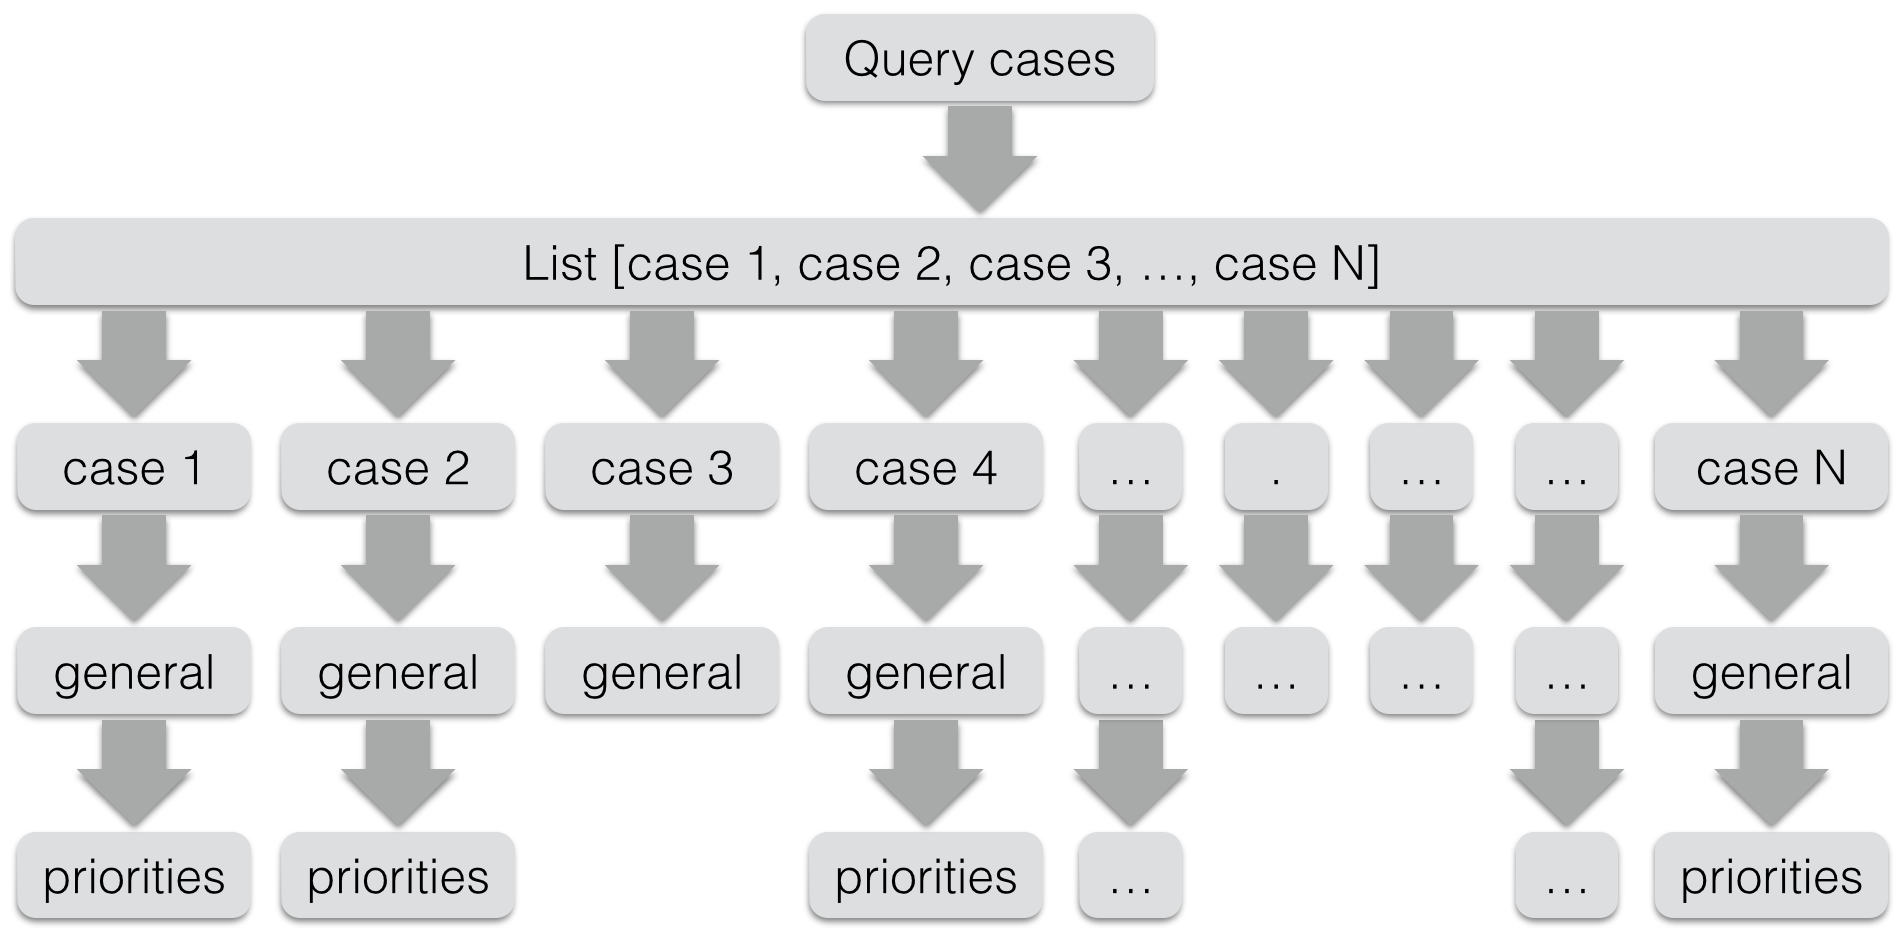
\includegraphics[width=0.9\textwidth]{images/streamflow_cases.png}
    \end{center}
  \caption{How the recursive requests are executed in the Streamflow web-client to fetch all needed resources and comply with HATEOAS.}
\end{figure}

By placing an API-gateway written with CrocodilePear in between the Streamflow web-client and the Streamflow API, all recursive requests can be concatenated for the client to one request with one response. By doing so, a lot of unnecessary data can also be discarded before it is sent to the client. This unnecessary data is duplicate data such as the duplicate case-information, irrelevant data for the client such as HATEOAS discovery information and unneeded data such as unused priorities.

In the test environment, measurements where made on a list which contained 156 cases. For this list, the client had to execute 373 requests (1 request for the list, 156 requests for each case to get the location of the general resource, 156 requests for the general resource for each case, and 60 priority requests for the cases which needed that information). All these request where replaced with one single request to the API-gateway which took care of the HATEOAS communication. By doing so, the load time for the client was reduced by 55\%, from 11 seconds to 5 seconds. The total transmitted data was reduced from 1,100 KB to 159 KB - a 86\% decrease of transmitted data.

The Streamflow API also doesn't compress the responses. By adding a gzip compression to the payload inside the API-gateway before responding to the client, the data could be reduced even more, from 1,100 KB to 9.9 KB, which amounts to a 99\% decrease of transmitted data!

In addition, the client transformed certain data types after retrieving it from the server so that it would fit in its internal model. For example, the field "dueOn" was truncated from "2015-02-17T23:59:59.000Z" to "2015-02-17" since the time was not relevant for the client. By utilising the API-gateway, these transformations could be taken care of before replying to the client. This means that no, potentially demanding and error prone, transformations had to be done on the client --- instead the data could be used directly from the response.

\begin{figure}[H]
  \centering
    \begin{center}
      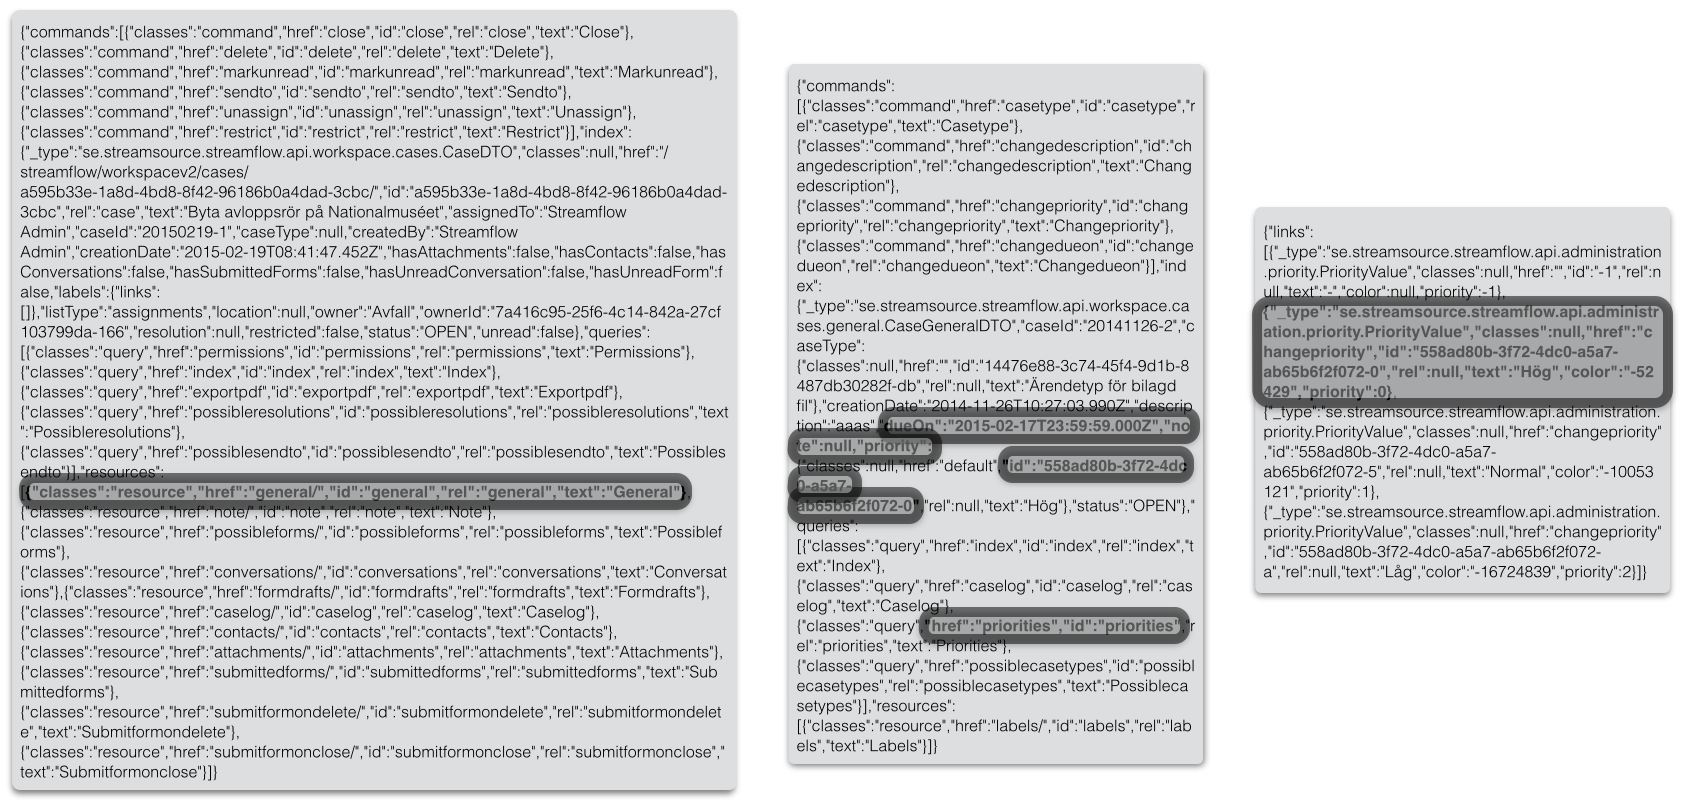
\includegraphics[width=0.9\textwidth]{images/streamflow_response.png}
    \end{center}
  \caption{Illustration of the responses (case, general and priorities) from Streamflow. The actual data needed in the list view is highlighted.}
\end{figure}

In the production environment, a measurement was made to determine the number of cases in the municipality of Jönköping at a given time of the day. On average, the number of cases in the non-empty inboxes where 19 and the maximum number of cases in one inbox where 296. This means that on average, the number of requests performed, every time an inbox is checked from the client, is roughly 40 - 60. When the largest inbox is viewed, the number of requests will be somewhere between 600 - 900 --- every time it is clicked. This is a substantial bottleneck for browsers on the HTTP/1.1 stack when looking at the TCP max-connection limit and various textual overheads.

It should be noted that the final version of the web-client will most likely be limited to displaying 10 - 20 cases at a time using pagination. This would reduce the number of requests to 20 - 60 for any given inbox view. This is however still a substantial amount of HTTP requests to perform every time a user checks an inbox. This approach will neither address the problem that 86\% of the transferred data is unnecessary overhead.

\cleardoublepage
\phantomsection
\addcontentsline{toc}{chapter}{Bibliography}
\bibliographystyle{plain}
\bibliography{anton_msc}

\begin{appendices}
\chapter{Definitions}
\section{JSON}
JSON, JavaScript Object Notation, is a data-interchange text format based on a subset of the JavaScript Programming Language. It is an open standard format which uses human-readable text. JSON is often used as an alternative to XML.

\section{XML}
XML, Extensible Markup Language, is a markup language used for encoding documents. It can be used as an alternative to JSON among many other document formats.

\section{REST}
REST, Representational State Transfer, consists of guidelines and best practices for creating scalable web services. The style was developed by W3C Technical Architecture Group (TAG) in parallel with HTTP/1.1. RESTful systems often communicate over HTTP using so called HTTP verbs such as GET, POST, PUT, DELETE to send and retrieve data between clients and servers.

\section{HATEOAS}
HATEOAS, Hypermedia as the Engine of Application State, is a constraint to the REST architecture. The clients enters a REST application through a fixed URL and all future actions are discovered dynamically within resource representations from the server.

\section{DMZ}

\end{appendices}

%\makebibliography{anton_msc}

\end{document}